%CLASSE DOCUMENTO - LINGUA E DIMENSIONE FONT
\documentclass[corpo=12pt,numerazioneromana]{toptesi}

%%%%%%%%%%%%%%%%%%%%%%%%%%%%%%%%%%%%%%%%%%%%%%%%%%%%%%%%%%%%%%%

% INCLUSIONE PACCHETTI
\usepackage[classica]{topfront}
\usepackage[utf8]{inputenc} %utf8
\usepackage[italian]{babel}
\usepackage[T1]{fontenc}
\usepackage{blindtext}
\usepackage{graphicx,wrapfig}
\usepackage{booktabs}
\usepackage{lmodern}
\usepackage{varioref}
\usepackage{url}
\usepackage{array}
\usepackage{paralist}{\obeyspaces\global\let =\space}
\usepackage{verbatim}
\usepackage{subfig}
\usepackage{tabularx}
\usepackage{amsmath}
\usepackage{amsfonts}
\usepackage{float}
\usepackage{amssymb}
\usepackage{multicol}
\usepackage{multirow}
\usepackage{listings}
\usepackage[]{geometry}
\geometry{a4paper, top=4.5cm, bottom=4.5cm, left=3.5cm, right=3.5cm, heightrounded, bindingoffset=5mm}
\usepackage[figuresright]{rotating}
\usepackage{algorithm}
\usepackage{algorithmic}
\usepackage{amsmath}
\usepackage[babel]{csquotes}
\usepackage{hyperref}
\usepackage[backend=biber,bibencoding=ascii]{biblatex}
\usepackage{xcolor}
\definecolor{seagreen}{rgb}{0.190, 0.525, 0.361}
\definecolor{darksalmon}{rgb}{0.914, 0.588, 0.478}
\newcommand{\MP}[1]{\textcolor{seagreen!100}{#1$_{_{\mathbf{MP}}}$}}
\newcommand{\MM}[1]{\textcolor{darksalmon!100}{#1$_{_{\mathbf{TP}}}$}}

%%%%%%%%%%%%%%%%%%%%%%%%%%%%%%%%%%%%%%%%%%%%%%%%%%%%%%%%%%%%%%%

% CONFIGURAZIONE LINK E RIFERIMENTI
\hypersetup{%
    pdfpagemode={UseOutlines},
    bookmarksopen,
    pdfstartview={FitH},
    colorlinks,
    linkcolor={black}, %COLORE DEI RIFERIMENTI AL TESTO
    citecolor={blue}, %COLORE DEI RIFERIMENTI ALLE CITAZIONI
    urlcolor={blue} %COLORI DEGLI URL
}

%%%%%%%%%%%%%%%%%%%%%%%%%%%%%%%%%%%%%%%%%%%%%%%%%%%%%%%%%%%%%%%

% CONFIGURAZIONE LISTATI/CODICE - CANCELLARE SE NON NECESSARIO
% PYTHON - BIANCO E NERO
\lstset{%
	captionpos=b,
	language=Python,
	basicstyle =\small\ttfamily,
	keywordstyle=\color{black}\bfseries,
	breaklines=true,
	breakatwhitespace=true,
	frame=lines,
	numbers=left,
	numberstyle=\footnotesize,
}

%%%%%%%%%%%%%%%%%%%%%%%%%%%%%%%%%%%%%%%%%%%%%%%%%%%%%%%%%%%%%%%

% FRENCHSPACING VA _SEMPRE_ ABILITATO PER DOCUMENTI IN ITALIANO
\frenchspacing

%%%%%%%%%%%%%%%%%%%%%%%%%%%%%%%%%%%%%%%%%%%%%%%%%%%%%%%%%%%%%%%

%DEFINIZIONE SEZIONI IN NUMERAZIONE ROMANA
%ELENCO DEI LISTATI/CODICI
\makeatletter
\newcommand\listofcodes{%
 \iffrontmatter\else\frontmattertrue\fi
 \if@openright\cleardoublepage\else\clearpage\fi
 % change the meaning of \chapter in a group
 \begingroup\def\chapter##1{\@schapter}
 \phantomsection % for the hyperlink
 \addcontentsline{toc}{chapter}{Elenco dei listati}
 \lstlistoflistings
 \endgroup
} 
\makeatother

\addto\captionsitalian{%
  \renewcommand{\lstlistlistingname}{Elenco dei listati}%
  \renewcommand{\lstlistingname}{Listato}%
}

%%%%%%%%%%%%%%%%%%%%%%%%%%%%%%%%%%%%%%%%%%%%%%%%%%%%%%%%%%%%%%%

% INFORMAZIONI PDF - PERSONALIZZARE
\pdfinfo{%
  /Title    (tesi magistrale-Erica Greco)
  /Author   (Erica Greco)
  /Subject  ()
  /Keywords (IMBH, pulsars, alberi decisionali )
}

%%%%%%%%%%%%%%%%%%%%%%%%%%%%%%%%%%%%%%%%%%%%%%%%%%%%%%%%%%%%%%%

% LISTA DEI CAPITOLI DA INCLUDERE - PERSONALIZZARE
\includeonly{%
intro,%
chap1,%
chap2,%
chap3,%
chap4,%
chap5,%
%app_a,%
}

% FILE DI BIBLIOGRAFIA
\addbibresource{bibliography.bib}

%%%%%%%%%%%%%%%%%%%%%%%%%%%%%%%%%%%%%%%%%%%%%%%%%%%%%%%%%%%%%%%

% INIZIO DOCUMENTO
\begin{document}

%%%%%%%%%%%%%%%%%%%%%%%%%%%%%%%%%%%%%%%%%%%%%%%%%%%%%%%%%%%%%%%

% FRONTESPIZIO - PERSONALIZZARE
%\frontespizio

\newgeometry{left=3.cm,right=3.cm,top=2.5cm,bottom=2.5cm}
%\centering
\begin{titlepage}
\begin{figure}
\centering

\includegraphics[scale=0.1]{images/Logo_Padova.png}
\end{figure}
\begin{center}
{{\Large{\textsc{Università degli Studi di Padova}}}}
\rule[0.1cm]{15.8cm}{0.05mm}
\rule[0.5cm]{15.8cm}{0.3mm}
{{\Large 
Dipartimento di Fisica e Astronomia Galileo Galilei}}\\
\vspace{3mm}
{{ 
Corso di Laurea magistrale in Astronomia}}
\end{center}

\vspace{18mm}
\begin{center}
\vspace{5mm}
{\LARGE{\bf Identificazione di buchi neri di massa}}\\
\vspace{3mm}
{\LARGE{\bf intermedia attraverso tecniche di machine }}\\
\vspace{3mm}
{\LARGE{\bf learning interpretabile }}\\
%\vspace{19mm} {\large{\bf Tesi di Laurea in Materia Tesi (opzionale)}}
\end{center}
\vspace{30mm}
\par
\noindent
\begin{minipage}[t]{0.47\textwidth}
{\large Relatore\\ \bf Prof.ssa Michela Mapelli}\\
\\
{\large Correlatore\\ \bf Dott. Mario Pasquato}

\end{minipage}
\hfill
\begin{minipage}[t]{0.47\textwidth} \raggedleft
{\large Laureanda\\ \bf Erica Greco}
\end{minipage}
\vspace{30mm}
%\par
%\noindent {\large{\bf Parole chiave:} Devono essere cinque... ma sono roba vecchia :-)}
\begin{center}
\large 24 Settembre 2020\smallskip\\
Anno Accademico 2019-2020
\end{center}
\end{titlepage}
\restoregeometry




%%%%%%%%%%%%%%%%%%%%%%%%%%%%%%%%%%%%%%%%%%%%%%%%%%%%%%%%%%%%%%%

%INTERLINEA - DEFAULT 1 - NON ESAGERATE, NON SUPERATE MAI 1.3 ;)
\interlinea{1.2}

%%%%%%%%%%%%%%%%%%%%%%%%%%%%%%%%%%%%%%%%%%%%%%%%%%%%%%%%%%%%%%%

\frontmatter

% DEDICA - PERSONALIZZARE
% VSPACE - PROPORZIONE USATA PER CENTRATURA VERTICALE DEL TESTO
% FLUSHRIGHT - ALLINEAMENTO ORIZZONTALE A DESTRA
\vspace*{\stretch{1}}
\begin{flushright}
\noindent
Dedica
\end{flushright}
\vspace*{\stretch{6}}
\cleardoublepage


% CITAZIONE - PERSONALIZZARE
% VSPACE - PROPORZIONE USATA PER CENTRATURA VERTICALE DEL TESTO
% FLUSHRIGHT - ALLINEAMENTO ORIZZONTALE A DESTRA
\vspace*{\stretch{1}}
\begin{flushright}
\noindent
Spazio per citazione

\textit{autore}
\end{flushright}
\vspace*{\stretch{6}}
\cleardoublepage

%%%%%%%%%%%%%%%%%%%%%%%%%%%%%%%%%%%%%%%%%%%%%%%%%%%%%%%%%%%%%%%

% RINGRAZIAMENTI - PERSONALIZZARE
\ringraziamenti
Spazio per ringraziamenti

%%%%%%%%%%%%%%%%%%%%%%%%%%%%%%%%%%%%%%%%%%%%%%%%%%%%%%%%%%%%%%%

% ABSTRACT - PERSONALIZZARE
\sommario
I modelli teorici indicano che gli ammassi globulari possano ospitare buchi neri di massa intermedia (\textit{Intermediate-Mass Black Holes}, IMBHs), ma i metodi osservativi usati finora non ne hanno ancora rilevato la presenza.

Rilevarli direttamente, infatti, può risultare difficoltoso con la strumentazione disponibile attualmente. Per questo motivo sono stati sviluppati metodi di identificazione indiretta. Uno di questi sfrutta l'informazione sul moto delle pulsar \cite{abbate1:paper} ed in questo lavoro di tesi si è cercato di applicarlo attraverso una tecnica innovativa. Nello specifico, ci si riferisce all'utilizzo di un modello di \textit{Machine Laerning} (ML) interpretabile: gli alberi decisionali di classificazione. In particolare, per costruire i \textit{dataset} forniti al modello ci si è serviti di un campione di simulazioni a N-corpi di ammassi globulari. Quest'ultimo è stato implementato in un codice in grado di classificare gli ammassi secondo la presenza di un IMBH al loro interno sulla base delle caratteristiche dinamiche delle pulsar. 

Si ottiene che l'albero decisionale allenato è in grado di classificare gli ammassi con il $70\%$ di accuratezza attraverso l'utilizzo delle proprietà dinamiche di sole 20 pulsar selezionate per ogni ammasso. 

Questo è solo un lavoro iniziale, infatti, il metodo può essere affinato e migliorato, ma nonostante questo presenta già dei risultati stimolanti per il futuro, in quanto sarebbe utile e innovativo applicarlo a dei dati reali.

%%%%%%%%%%%%%%%%%%%%%%%%%%%%%%%%%%%%%%%%%%%%%%%%%%%%%%%%%%%%%%%

% INDICI - ELIMINARE GLI INDICI NON NECESSARI

% INDICE GENERALE
\tableofcontents

% INDICE DELLE FIGURE
%\listoffigures

% INDICE DELLE TABELLE
%\listoftables

% INDICE DEI CODICI
%\listofcodes

%%%%%%%%%%%%%%%%%%%%%%%%%%%%%%%%%%%%%%%%%%%%%%%%%%%%%%%%%%%%%%%

\mainmatter

% INCLUSIONE FILE CAPITOLI - PERSONALIZZARE - TENERE COERENTE CON LISTA IN ALTO
\chapter*{Introduzione}
\addcontentsline{toc}{chapter}{Introduzione}
\label{chap:intro}
I buchi neri di massa intermedia (\textit{Intermediate-Mass Black Holes}, IMBHs) sono buchi neri la cui massa è compresa tra $10^{2}$ e $10^{6}M_{\odot}$. Si pensa che essi possano essere l'anello mancante necessario per collegare le informazioni note riguardanti i buchi neri di origine stellare ($\sim 10 M_{\odot}$) a quelle riguardanti i buchi neri super-massicci ($10^{6}-10^{10}M_{\odot}$). Infatti, i modelli teorici prevedono l'esistenza degli IMBHs al centro di ammassi globulari (\textit{Globular Cluster}, GC), mentre le osservazioni condotte finora non ne hanno ancora rilevato la presenza \MP{a parte il recentissimo evento di detection di onde gravitazionali GW190521, che viene intepretato come la formazione di un buco nero di $\approx 150$ masse solari \cite{Abbott2020:paper}, quindi in ogni caso di massa abbastanza vicina all'estremo stellare del range di massa degli IMBH}. 

La motivazione per cui questi oggetti peculiari risultano sfuggenti rispetto ai buchi neri appartenenti alle altre categorie è legata principalmente al fatto che la strumentazione attuale presenti dei limiti in tal senso.  
Tuttavia, esistono dei metodi indiretti per poter identificare gli IMBHs negli ammassi. Uno fra essi è quello che si basa sulla dinamica delle MSPs nei GCs. In particolare, attraverso misure delle derivate dei periodi delle MSPs sarebbe possibile ottenere i loro valori di accelerazione e delle sue derivate: il \textit{jerk} (derivata prima dell'accelerazione) e lo \textit{snap} (derivata seconda dell'accelerazione). Dallo studio di tali caratteristiche, poi, si potrebbe risalire all'identificazione degli IMBHs \cite{abbate1:paper}. 

A partire da questa proposta, questo lavoro si sviluppa verso tale scopo, ma utilizzando metodi diversi. Infatti, vengono utilizzate tecniche di \textit{Machine Learning} interpretabile per prevedere la presenza di IMBHs al centro di GCs. 

Poiché i dati osservativi in questo campo non sono sufficienti, per lo studio si sono utilizzati dati ottenuti da un set di simulazioni a N-corpi. Il modello di \textit{Machine Learning} utilizzato è quello degli alberi decisionali, caratterizzati dalla possibilità di essere interpretati. Questa è un' importante caratteristica per un modello previsionale che riguarda soprattutto la fase di analisi dei risultati. 

Gli ammassi simulati sono stati classificati dal modello secondo la presenza di un IMBH o meno sulla base delle caratteristiche dinamiche delle MSPs scelte nelle regioni centrali dei GCs. Nello specifico, le caratteristiche fornite al modello sono: la distanza delle MSPs dal centro di massa del GC proiettata sul piano del cielo e le componenti di velocità, accelerazione, \textit{jerk} e \textit{snap}, considerate lungo la linea di vista. 

La ricerca di IMBHs attraverso questo metodo potrebbe essere una nuova strada alternativa da percorrere per ottenere dei risultati soddisfacienti, specie se tali metodi in futuro potranno essere applicati a dati reali.

Il lavoro di tesi può essere suddiviso principalmente in tre parti. La prima e la seconda parte  si sviluppano rispettivamente nei capitoli \ref{chap:cap1} e \ref{chap:cap2}. La terza parte, invece, contiene i restanti tre capitoli.\\
Nel primo capitolo viene presentato e contestualizzato il problema astrofisico su cui si basa l'intera tesi: la ricerca degli IMBHs in ammassi globulari. Viene, dunque, fornita un'introduzione sugli IMBHs e su quali sono i metodi utilizzati finora per identificarli, per poi concentrarsi, in particolare, sul metodo delle MSPs.\\
Nel secondo capitolo, invece, viene descritto lo strumento utilizzato per lo sviluppo del progetto, ovvero gli alberi decisionali. Dopo una breve introduzione al \textit{Machine Learning}, viene descritto l'algoritmo CART \cite{brei:book} che è quello utilizzato per la costruzione degli alberi decisionali in questo lavoro. Vengono, infatti, descritte le fasi in cui l'algoritmo si sviluppa e le metodologie che esso adopera, come, ad esempio, la tecnica del \textit{pruning} utilizzata in questo caso per risolvere un problema comune a tutti gli algoritmi di \textit{Machine Learning}: il problema dell'\textit{overfitting}. Inoltre, in questo capitolo, vengono forniti gli strumenti per valutare le prestazioni di un algoritmo di classificazione.\\
Infine, nell'ultima parte si entra nel merito del lavoro di tesi descrivendo nello specifico i \textit{dataset} utilizzati, il codice sviluppato per la classificazione degli ammassi (Cap. \ref{chap:cap3}) e, in ultimo, vengono presentati i risultati ottenuti con la relativa interpretazione (Cap. \ref{chap:cap4}). Nel quinto ed ultimo capitolo, invece, vengono discusse le conclusioni e presentate le possibili prospettive future per l'identificazione di IMBHs in GCs attraverso tecniche di \textit{Machine Learning}.







\chapter{A caccia di buchi neri di massa intermedia}
\label{chap:cap1}

In questo Capitolo viene presentato il \textit{background} astrofisico sul quale si sviluppa l'intero lavoro di tesi.\\
Ci si focalizza sull'importanza di voler ricercare i buchi neri di massa intermedia (\textit{Intermediate-Mass Black Holes}, IMBHs) all'interno degli ammassi globulari (\textit{Globular Clusters}, GCs) e vengono presentate alcune tecniche utilizzate per la loro identificazione. In particolare, viene approfondito il metodo di identificazione basato sulla dinamica delle Pulsar Millisecondo (\textit{Millisecond Pulsars, MSPs}) all'interno dei GCs. Infatti, questo progetto si sviluppa in una direzione diversa, ma complementare all'idea suggerita da Abbate el al.(2019) \cite{abbate1:paper} di identificare gli IMBHs nei GCs utilizzando, oltre alle velocità e accelerazioni delle MSPs in ammasso, anche le informazioni dinamiche fornite dalle derivate dell'accelerazione.\\
Nello specifico, nella mia tesi, ho sviluppato un codice che utilizza un modello di \textit{Machine Learning} (ML) interpretabile in grado di fare previsioni sulla presenza di IMBHs in ammassi sulla bese di tali informazioni dinamiche delle MSPs.

\section{I buchi neri di massa intermedia}
\label{sec:IMBH}
I buchi neri vengono classificati in base alla loro massa in: buchi neri di origine stellare, buchi neri di massa intermedia e buchi neri super-massicci.\\
I buchi neri di origine stellare sono oggetti compatti che si formano alla fine della vita di stelle massicce in seguito ad esplosioni di Supernova, mentre i buchi neri super-massicci normalmente si trovano al centro di galassie. I buchi neri di massa intermedia, invece, (\textit{Intermediate-Mass Black Holes}, IMBHs) sono buchi neri la cui massa (tra 100 e $10^{6}$ M$_{\odot}$) è significativamente maggiore di quella dei buchi neri di origine stellare e al contempo molto minore di quella dei buchi neri super-massicci.

I buchi neri sono caratterizzati da intensi campi gravitazionali dai quali, escludendo fenomeni quantistici non ancora verificati sperimentalmente, nulla può fuoriuscire, nemmeno la radiazione. Per questo motivo non possono essere osservati direttamente, ma possiamo unicamente misurare gli effetti che essi hanno sugli altri corpi celesti. Ad esempio, è possibile rilevare le emissioni X quando essi, in un sistema binario, accrescono sottraendo massa ad una stella compagna (Fig.\ref{fig:binario}) o le emissioni sottoforma di onde gravitazionali quando si fondono (fenomeno di \textit{merging}) con altri oggetti compatti o anche si possono rilevare gli effetti gravitazionali che hanno sulle orbite di altri oggetti, come nel caso di un buco nero super-massivo nel centro galattico.
\begin{figure}
\begin{center}
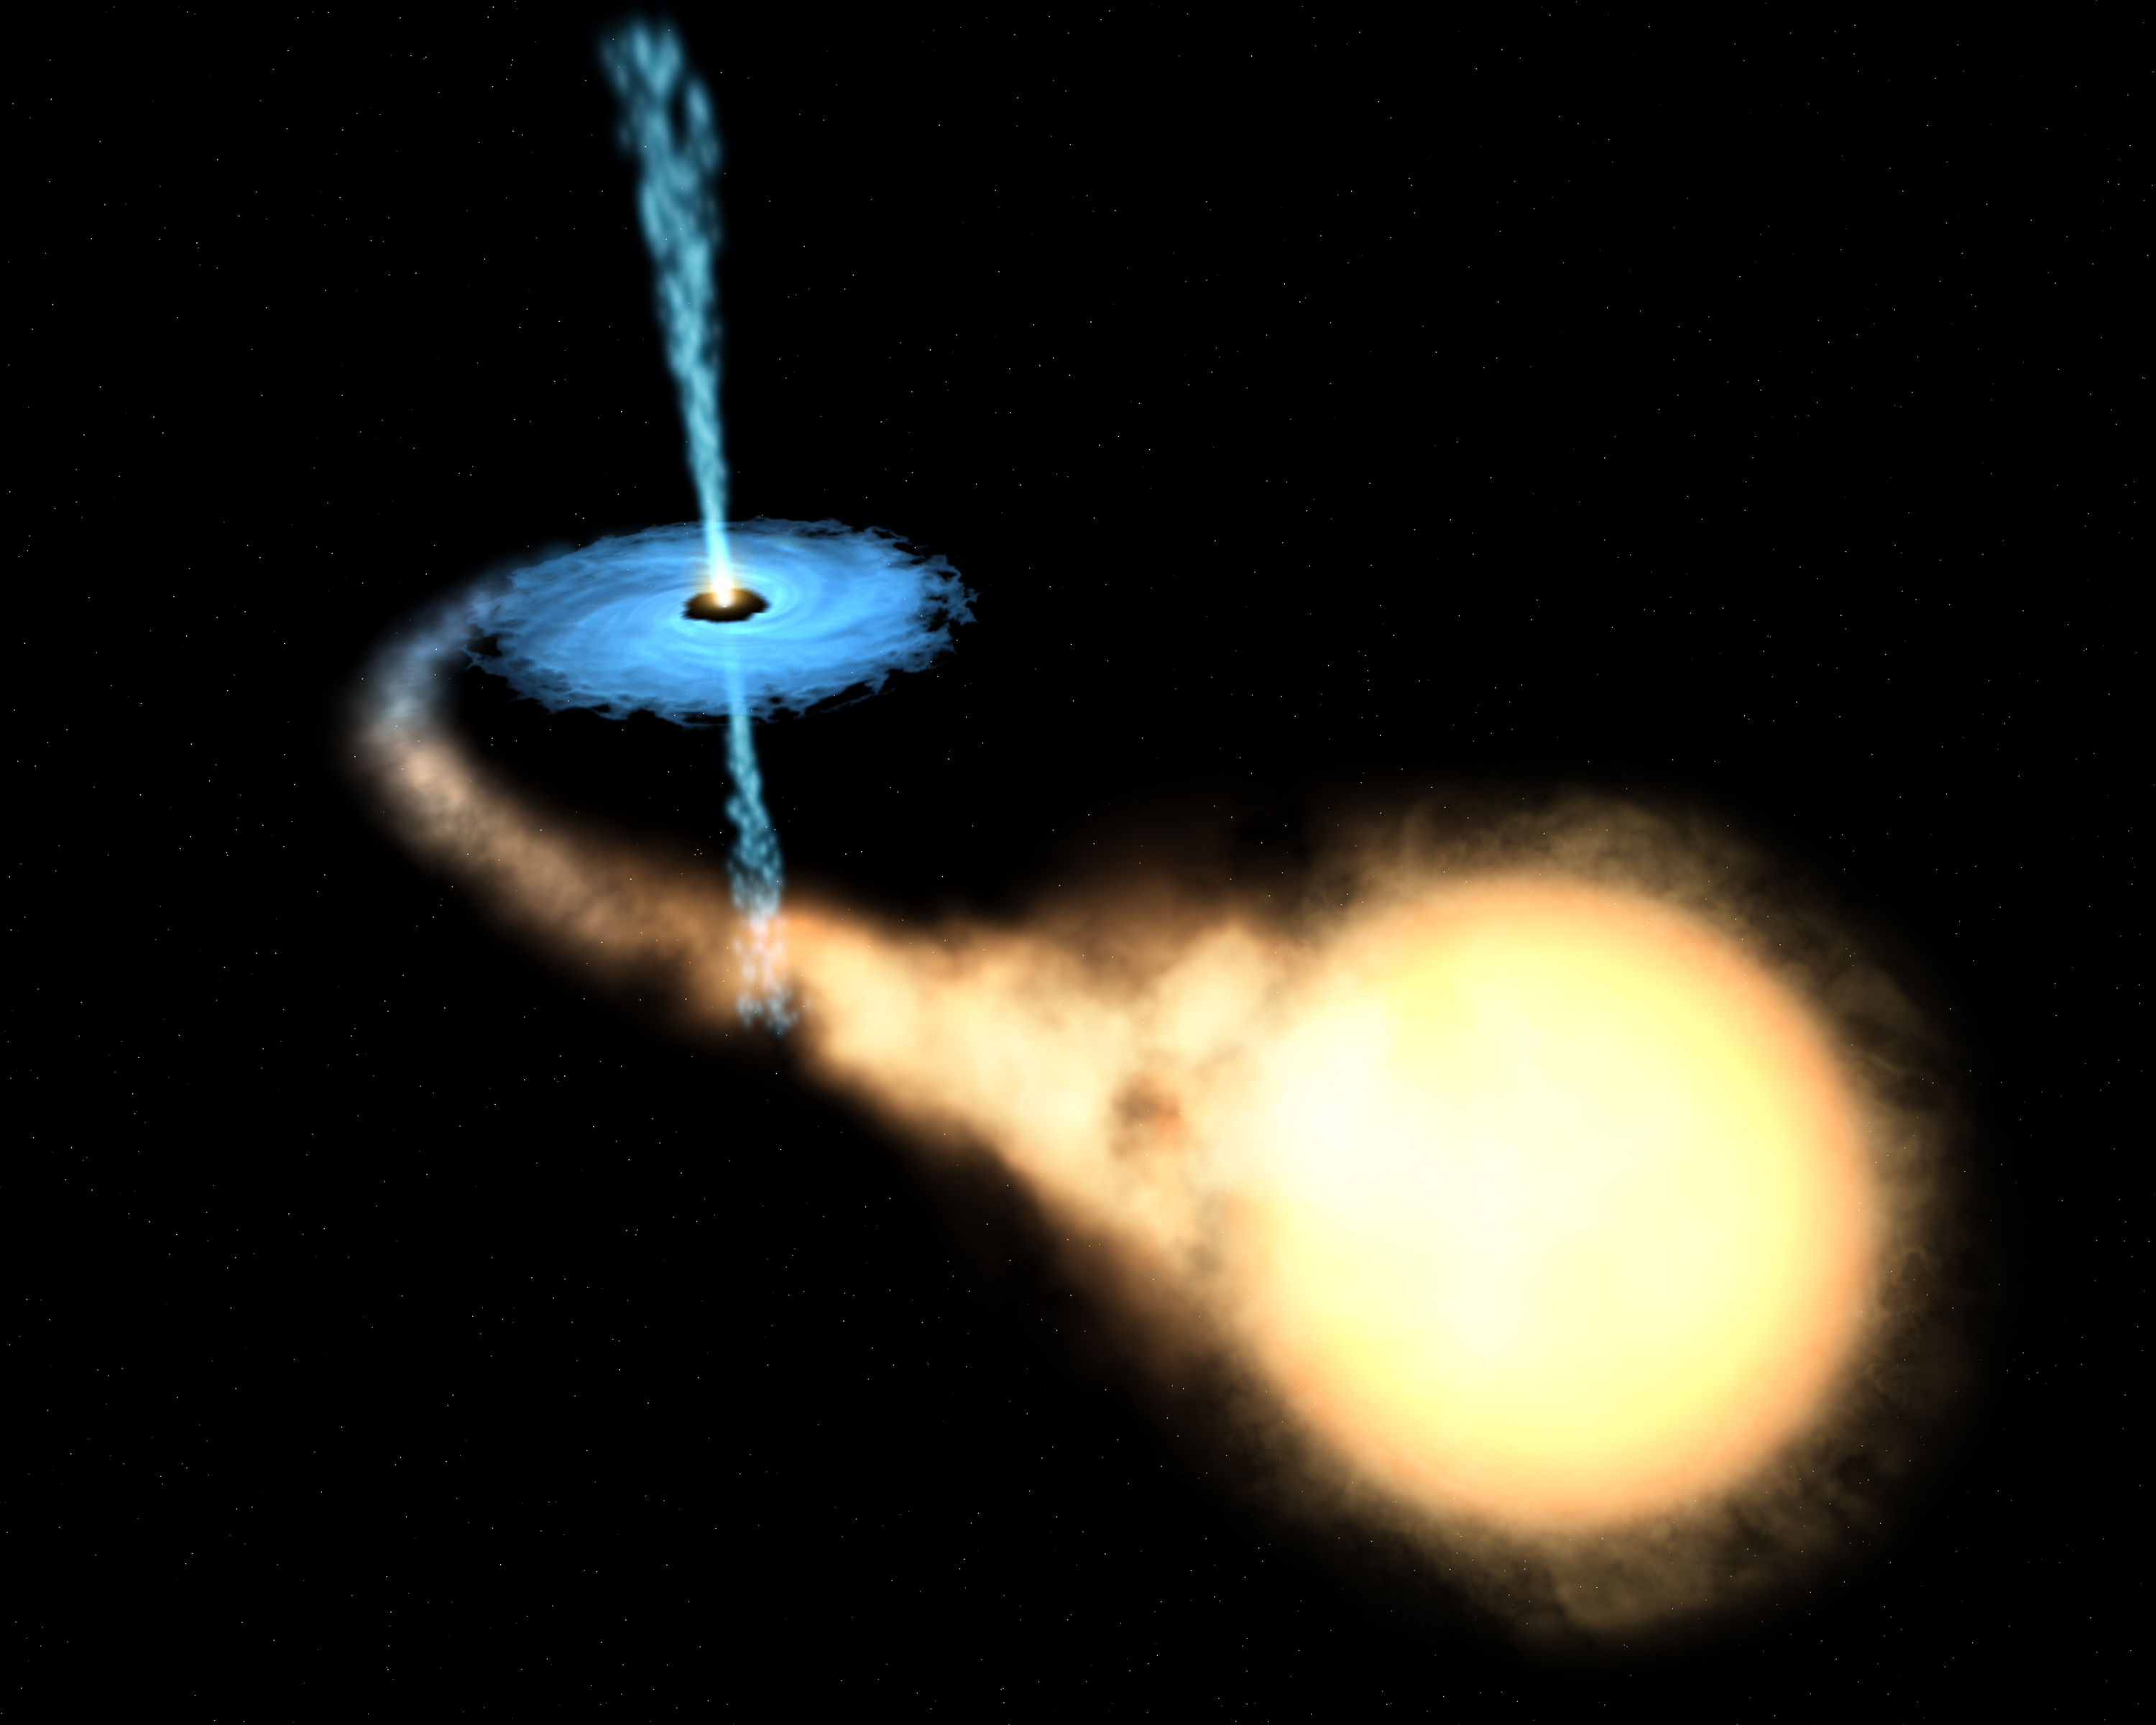
\includegraphics[width=0.4\columnwidth]{images/Accretion_disk.jpg}
\end{center}
\caption{Esempio, in un \textit{artist impression}, di buco nero in un sistema binario che accresce la propria massa a discapito della sua stella compagna \cite{binaria:online}.}
\label{fig:binario}
\end{figure}

Gli IMBHs, oggetto di studio di questa tesi, dal punto di vista osservativo, potrebbero rappresentare il nesso che collega le informazioni raccolte finora e che riguardano principalmente i buchi neri di origine stellare e quelli super-massici. Infatti, nonostante i modelli teorici suggeriscano fortemente che è possibile trovare gli IMBHs all'interno di ammassi globulari \cite{milham:paper}, attualmente non si dispone di prove definitive per confermarlo, in quanto gli indizi che abbiamo sono ancora relativamente controversi e non si è ancora raggiunto il consenso presso la comunità scientifica (Fig.\ref{fig:imbh_gap}).
\begin{figure}[H]
\begin{center}
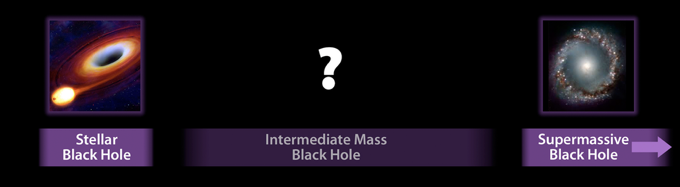
\includegraphics[width=0.7\columnwidth]{images/IMBH_gap.png}
\end{center}
\caption{Vuoto di informazioni tra le categoria di buchi neri di origine stellare ed i buchi neri super-massivi: gli IMBHs.}
\label{fig:imbh_gap}
\end{figure}

Gli scenari di formazione proposti per questi oggetti peculiari sono molteplici \cite{jenny:paper}.\\
Il primo scenario ipotizza che gli IMBHs possono essersi originati in seguito al collasso di stelle di Popolazione III, ovvero ipotetiche stelle formatesi con abbondanza chimica primordiale che possono raggiungere alte masse rispetto alle stelle odierne \cite{abel:paper}.\\
La seconda ipotesi è quella del collasso diretto secondo cui la loro massa si sarebbe addensata direttamente dal materiale dell’universo in formazione subito dopo il \textit{Big Bang}, senza passare per le fasi dell'evoluzione stellare \cite{haehnelt:paper}.\\
Un ultimo interessante scenario, invece, suggerisce che essi si formino mediante fenomeni di collisione e di \textit{merging}. In questo caso esistono più ipotesi.\\ 
Secondo \textit{Miller $\&$ Hamilton 2002} \cite{milham:paper} un buco nero di origine stellare di 50 $M_{\odot}$ potrebbe collocarsi in breve tempo al centro dell’ammasso per l'effetto di segregazione di massa; successivamente, collisioni con altri buchi neri stellari mediate da incontri gravitazionali a tre e quattro corpi e da perdita di energia per emissione di onde gravitazionali, porterebbero al raggiungimento di masse dell’ordine di $10^{3}$ $M_{\odot}$ in un tempo paragonabile a quello di Hubble.\\
Un altro meccanismo, invece, propone che in un $core$ ad alta densità, le stelle molto massicce $\left(50-100 M_{\odot}\right)$ possono essere soggette ad un’efficiente segregazione di massa che le colloca nel nucleo dell’ammasso mentre si trovano in fase di Sequenza Principale. A questo punto si verificherebbe un numero sempre crescente di collisioni e \textit{merging} tra stelle che porterebbero alla formazione e all’immediato collasso di una stella con massa pari a $\simeq 10^{-3}$ volte la massa dell'ammasso, generando così un IMBH \cite{portzw:paper}.\\
I GCs, essendo ambienti stellari densi e dinamicamente attivi, potrebbero essere i luoghi ideali per la formazione di IMBHs attraverso collisioni stellari o incontri gravitazionali tra buchi neri  di origine stellare e successive fusioni \cite{portmcmil:paper}. L'interesse per la formazione di IMBHs in GCs è anche legato al fatto che gli ammassi globulari più massicci tendono a precipitare rapidamente verso il centro della galassia, dove potrebbero concorrere a formare il \textit{nuclear star cluster} \cite{arcasedda:paper}. Pertanto, essi rappresentano un possibile meccanismo di formazione di un buco nero super-massivo attraverso fenomeni di \textit{merging} tra IMBHs.

In condizioni di prossimità ad una binaria di oggetti compatti gli IMBHs possono essere sorgenti di emissione di onde gravitazionali.\\ 
Gli interferometri terrestri di onde gravitazionali LIGO e Virgo \cite{ligo:online}, \cite{virgo:online}, \cite{ligovirgo1:paper} operano in un intervallo di frequenze tra 
qualche decina e qualche migliaio di Hertz. Quindi possono osservare la coalescenza di buchi neri fino ad una massa di
$\sim 500 M_{\odot}$, nel regime degli IMBHs.\\ 
La prossima generazione di interferometri nello
spazio, come il Laser Interferometer Space Antenna, LISA \cite{amaro:paper}, sarà ancora più adatta ad osservare gli IMBHs, poiché opererà nel range di frequenza compreso tra $10^{-3}-10^{-1}$ Hertz.\\
Inoltre, gli IMBHs sono molto difficili da individuare in quanto, gli ammassi globulari sono ambienti decisamente poveri di gas, poiché sono costituiti principalmente da stelle vecchie e il gas primordiale che era presente è stato utilizzato nelle precedenti fasi di formazione stellare o spazzato via da esplosioni di Supernova. Per tale ragione e per come operano i meccanismi di accrescimento, ovvero tramite la dissipazione di energia e momento angolare verso l'esterno di un disco, risulta difficile rilevare emissioni X, determinate da tali fenomeni.\\
Un'altra ragione per cui risulta difficoltoso rilevarli è legata alla componente stellare.\\
Per ogni buco nero di massa $M_{BH}$, infatti, è possibile stimare il raggio di influenza $r_{i}$:
\begin{equation}
r_{i}=\frac{G M_{B H}}{\sigma^{2}}
\label{eq:rinfl}
\end{equation}
con $G$ la costante di gravitazione universale e $\sigma$ la dispersione di velocità delle stelle subito al di fuori della sfera di influenza del buco nero. Le stelle all’interno di questo raggio risentono principalmente dell’influenza gravitazionale del buco nero stesso.\\
Il raggio di influenza di un IMBH è dell'ordine di solo qualche secondo d'arco. Ad esempio, un IMBH di $\sim1000M_{\odot}$ all'interno di \textit{47 Tucanae} avrebbe un raggio di influenza di circa $1"$ \cite{jenny:paper}, contro la dimensione apperente dell'ammasso di circa 31' \cite{47tuc:online}. Pertanto, in generale, la sfera di influenza di un IMBH non è così importante, rispetto alle dimensioni dell'ammasso, da influenzare gravitazionalmente un numero di stelle sufficientemente elevato da determinare una quantità di eventi di accrescimento mareale tale da poter essere osservato. 

\section{Metodi di identificazione di IMBHs al centro di ammassi globulari}
\label{sec:identificazione}

Di fronte alla presenza di un IMBH in un ammasso stellare, ci aspettiamo che si verifichino delle alterazioni nei profili di densità del GC e di dispersione di velocità delle stelle dell'ammasso. Sulla base di questi si costruiscono la maggior parte dei metodi di identificazione degli IMBHs con le relative difficoltà a livello pratico. Inoltre, se ci trovassimo in presenza di un fenomeno di accrescimento, la misurazione delle emissioni X e radio sarebbe un altro canale identificativo di IMBH al centro di un GC \cite{strader:paper}.

Un IMBH aumenta la profondità della buca di potenziale di un ammasso causando un incremento della densità stellare nelle zone centrali. Queste ultime, pertanto, risultano avere un profilo di densità di una \textit{cuspide} ben descritta dalla legge di potenza $\rho \propto r^{-\alpha}$, con $\alpha \simeq 1.55$ \cite{baum:paper}.  

Le stelle all’interno del raggio di influenza $r_{i}$ (eq. \ref{eq:rinfl}) del IMBH, oltre a risentire principalmente dell’influenza gravitazionale del buco nero, seguono un profilo di dispersione di velocità di tipo \textit{kepleriano} caratterizzato da una ripidità nelle regioni centrali. Tuttavia, la determinazione accurata della dispersione di velocità delle stelle valutata solo nella regione centrale del GC, è al limite delle capacità dell’attuale strumentazione astronomica e richiede un’elevatissima risoluzione spaziale. I risultati di misurazioni effettuate con metodi diversi (spettroscopia in luce integrata, stelle individuali, studio dei moti propri) sono talvolta in disaccordo tra loro, con la conseguenza che la comunità scientifica non ha ancora raggiunto un consenso in merito \cite{lutz1:paper}.\\
Il profilo di dispersione di velocità, però si può ottenere teoricamente sulla base del profilo di densità determinato precedentemente e considerando un oggetto puntiforme di una certa massa al centro dell’ammasso \cite{lutz:paper}.\\
Come risultato si ottiene una famiglia di profili di dispersione di velocità che, una volta confrontati con le osservazioni, restituiscono la massa del BH centrale (Fig.\ref{fig:profili_vel}).
\begin{figure}[ht]
\begin{center}
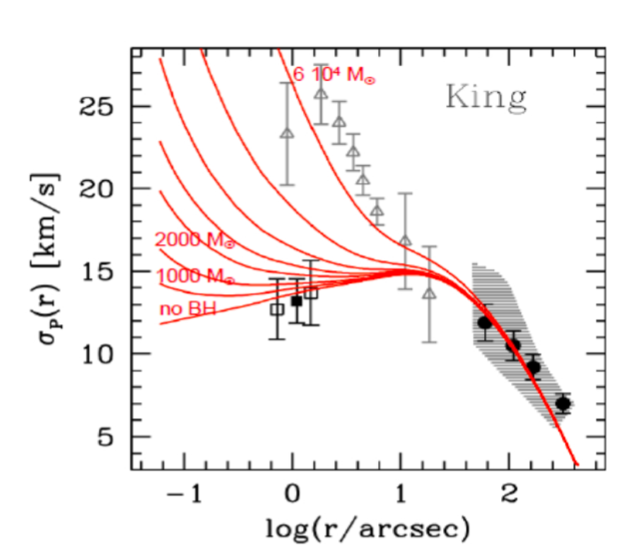
\includegraphics[width=0.6\columnwidth]{images/profili_vel.png}
\end{center}
\caption{Profilo di dispersione di velocità osservato per l'ammasso globulare NGC 6388 con sovrapposte le linee rosse continue delle famiglie di modelli considerate. Esse sono state ottenute assumendo una diversa massa per il buco nero centrale. Si noti che aumentando la massa del IMBH la pendenza nelle regioni centrali risulta più ripida \cite{Lanzoni:paper}, \cite{lutz:paper}.}
\label{fig:profili_vel}
\end{figure}

Tuttavia, la presenza di una \textit{cuspide} nelle regioni centrali di un GC può essere dovuta anche a cause diverse dalla presenza di un IMBH. Ad esempio, a seguito di un collasso del \textit{core}, tanti buchi neri di massa stellare potrebbero trovarsi nelle regioni centrali dell'ammasso e determinare, quindi, i ripidi profili di velocità e densità associati alle cuspidi \cite{trenti:paper}. Questo vuol dire, in altre parole, che la presenza di una cuspide non è sufficiente per affermare che al centro dell'ammasso ci sia un IMBH. Ma anche il viceversa non è sufficiente per affermare il contrario. Infatti, la non rilevazione di una cuspide non esclude a priori la presenza di un IMBH centrale. Come abbiamo già visto, infatti, la sfera di influenza di un IMBH potrebbe rivelarsi decisamente troppo piccola per far sì che la cuspide si veda.

Oltre ai metodi che si servono della dinamica stellare in ammasso e dei moti propri delle stelle \cite{banwolf:paper}, \cite{gebh:paper}, un altro metodo per l'dentificazione degli IMBH potrebbe essere quello che si basa sul rilevamento dell'emissione X e radio degli IMBHs in fase di accrescimento \cite{mac1:paper}, \cite{mac2:paper}.\\
Tali emissioni, però, risultano difficili da osservare nei GCs poichè si tratta di sistemi poveri di gas. Tuttavia, recentemente, le prove dell'esistenza di un IMBH in un GC potrebbero essere fornite dall'osservazione di un evento di disturbo di marea in un ammasso extra-galattico \cite{lin:paper}. I dati in X sono stati raccolti dai telescopi in orbita \textit{Chandra} e \textit{XMM-Newton} e successivamente confermati dal \textit{Telescopio Spaziale Hubble}. Attualmente si stanno svolgendo ulteriori indagini osservative per identificare la natura dell'oggetto responsabile dell'evento, ma gli autori dello studio, \textit{Lin D. et al. 2020} \cite{lin_2020:paper}, sostengono si tratti di un IMBH in procinto di inglobare una stella.\\
\indent
Oltre a questi, esistono anche metodi indiretti per rilevare IMBH al centro di ammassi. Uno tra questi è quello che si basa sull'effetto degli IMBHs sulla segregazione di massa \cite{pasquato:paper}. Nei GCs, ci si aspetta, infatti, che gli IMBHs per la maggior parte del tempo si trovino in sistemi binari con altri oggetti massicci, come buchi neri di origine stellare. In questa configurazione essi inietterebbero energia nel nucleo del GC, attenuando la segregazione di massa stellare. Anche le binarie primordiali, però, potrebbero essere responsabili dello stesso fenomeno. Ciò porterebbe ad un problema di degenerazione nell'indicatore di segregazione di massa, che potrebbe essere risolto misurando la frazione di binarie nel \textit{core} in maniera indipendente. Questo, però, ha le sue complicazioni dovute ai problemi di risoluzione spaziale di cui si è già parlato. Anche per questo motivo gli studi portati avanti sulla base di tale metodologia non sono ancora stati in grado di rilevare forti candidati di GCs che ospiterebbero un IMBH.

Tutti i metodi presentati riscontrano delle difficoltà nell'identificazione degli IMBHs all'interno degli ammassi. Queste sono legate soprattuto ai fattori che ne influenzano la rilevazione diretta. Gli IMBHs, infatti, risultano così sfuggenti principalmente a causa dei problemi che comporta la piccola dimensione della loro sfera di influenza e, conseguentemente, dei problemi osservativi relativi alla risoluzione spaziale per i \textit{core} degli ammassi.
Per tali ragioni risulta interessante approfondire un metodo alternativo e indiretto per la ricerca di IMBHs all'interno di ammassi globulari: quello che si basa sullo studio delle proprietà dinamiche delle Pulsar Millisecondo (\textit{Millisecond Pulsars, MSPs}) \cite{pere:paper}, \cite{abbate:paper}.  
I paragrafi successivi, infatti, saranno dedicati all'approfondimento di tale metodo che è proprio quello su cui si basa questo progetto di tesi.

\section{Metodo delle MSPs}
\label{sec:MSP}

Le MSPs sono oggetti molto frequenti nei GCs ed essendo caratterizzate da periodi di rotazione estremamente stabili, possono essere utilizzate come strumento per l'identificazione di IMBHs all'interno di ammassi globulari. Infatti, le misure ottenute per effetto Doppler permettono di avere informazioni sulle loro accelerazioni e sulle derivate temporali di ordine superiore.\\
In particolare, le derivate prima, detta \textit{jerk}, e seconda, detta \textit{jounce} o \textit{snap}, dell'accelerazione delle MSPs in ammassi, sono state valutate in maniera più approfondita nel recente articolo di Abbate et al. (2019) \cite{abbate1:paper}.\\
\MP{Pero l'articolo di Abbate e puramente simulativo; andrebbe scovata una referenza osservativa su che cosa si puo veramente misurare sulle pulsar reali}
\subsection{Profili radiali di Jerk e Snap in ammasso}
\label{subsec:profili}

Analiticamente è possibile derivare le relazioni matematiche che descrivono i profili radiali di \textit{jerk} e \textit{snap} di stelle in ammasso \cite{abbate1:paper}.

Consideriamo una stella di prova che sperimenta l'attrazione gravitazionale del campo generato da tutte le stelle dell'ammasso, in particolare assumiamo che il GC sia descritto dal profilo di King \cite{king:paper}.\\
L'accelerazione in funzione della distanza \textit{r} dal centro dell'ammasso, nelle regioni centrali del GC, può essere approssimata come:
\begin{equation}
   \textbf{a}(r) = -4 \pi G \rho_{c} r_{c}^{3} \left[\sinh^{-1} \left(\frac{r}{r_{c}}\right) - \frac{r}{r_{c}\sqrt{1+({r}/{r_c})^{2}}}\right] \frac{\textbf{r}}{r^{3}} = -\left | a \right | \frac{\textbf{r}}{r}
   \label{eq:accrad_king}
\end{equation}
dove $\rho_{c}$ è la densità centrale dell'ammasso ed $r_{c}$ il raggio del $core$.\\
Per calcolare il $jerk$ è necessario derivare rispetto al tempo l'equazione \ref{eq:accrad_king}, ottenendo:
\begin{equation}
\mathbf{\Dot{a}}_{K}(r)=-\frac{d|a(r)|}{d t} \frac{\mathbf{r}}{r}-|a(r)| \frac{\mathbf{v}}{r}+|a(r)| \frac{(\mathbf{v} \cdot \mathbf{r}) \mathbf{r}}{r^{3}}
\label{eq:jerk_king}
\end{equation}
in cui la derivata temporale della norma dell'accelerazione è data da:
\begin{equation}
\frac{d|a(r)|}{d t}=-2 \frac{v|a(r)|}{r}+4 \pi G v \rho_{\mathrm{c}}\left(\frac{1}{1+\left(r / r_{\mathrm{c}}\right)^{2}}\right)^{\frac{3}{2}}
\end{equation}
con $v$ la norma della velocità.\\
Nel caso in cui il GC fosse caratterizzato da forti fenomeni di collisioni stellari, anche i $jerk$ potrebbero risultare influenzati dalle stelle vicine. In questo caso, il $jerk$ sarebbe caratterizzato dalla seguente distribuzione di probabilità \cite{prager:paper}:
\begin{equation}
P(\dot{a})=\frac{1}{\pi^{2}} \frac{\dot{a}_{0}}{\left(\dot{a}^{2}+\dot{a}_{0}^{2}\right)^{2}}
\end{equation}
in cui $\dot{a}_{0}$ è il $jerk$ caratteristico dato da:
\begin{equation}
\dot{a}_{0}=\frac{2 \pi \xi}{3} G\langle m\rangle \sigma n
\end{equation}
dove $\xi$=3.04 è una costante numerica, $\langle m \rangle$ è la massa media delle stelle, $\sigma$ è la dispersione di velocità ed $n$ è la densità numerica delle stelle.\\
La distribuzione dei $jerk$ proiettata lungo la linea di vista $\dot{a}_{l}$ è una distribuzione Lorentziana:
\begin{equation}
P\left(\dot{a}_{l}\right)=\frac{1}{\pi} \frac{\dot{a}_{0}}{\dot{a}_{l}^{2}+\dot{a}_{0}^{2}}
\end{equation}
Se all'interno del GC vi è un IMBH, il $jerk$ della stella di prova sarà influenzato dalla massa centrale $M$ ed il profilo sarà:
\begin{equation}
\dot{\mathbf{a}}_{M}=-G M\left(\frac{\mathbf{v}}{r^{3}}-3 \frac{(\mathbf{v} \cdot \mathbf{r}) \mathbf{r}}{r^{5}}\right)
\label{eq:jerk_imbh}
\end{equation}
dove \textbf{r} è la distanza dalla massa $M$ e \textbf{v} è la relativa velocità.\\
Inoltre l'IMBH crea una sovra-densità stellare caratterizzata da un profilo radiale con \textit{slope} pari a -1.55 \cite{baum:paper}:
\begin{equation}
\dot{\mathbf{a}}_{\mathrm{cusp}}=\left\{\begin{array}{l}
-\frac{4 \pi G}{1.45} r_{\mathrm{i}}^{1.55} \rho_{\mathrm{i}}\left(\frac{\mathrm{v}}{r^{1.55}}-1.55 \frac{(\mathrm{v} \cdot \mathrm{r}) \mathrm{r}}{r^{3.55}}\right) \text { for } r<r_{\mathrm{i}} \\
-\frac{4 \pi G}{1.45} r_{\mathrm{i}}^{3} \rho_{\mathrm{i}}\left(\frac{\mathrm{v}}{r^{3}}-3 \frac{(\mathrm{v} \cdot \mathrm{r}) \mathrm{r}}{r^{5}}\right) \text { for } r>r_{\mathrm{i}}
\end{array}\right.
\label{eq:jerk_cusp}
\end{equation}
in cui $r_{i}$ è il raggio di influenza dell'IMBH e $\rho_i$ è il valore di densità a tale raggio.

Derivando rispetto al tempo le equazioni \ref{eq:jerk_king}, \ref{eq:jerk_imbh} e \ref{eq:jerk_cusp} è possibile ottenere anche i profili radiali degli $snap$ all'interno degli ammassi.\\
Il contributo del campo gravitazionale dell'intero ammasso è dato dalla:
\begin{equation}
\begin{aligned}
\ddot{\mathbf{a}}_{K}&=-\frac{d^{2}|a(r)|}{d t^{2}} \frac{\mathbf{r}}{r}-2 \frac{d|a(r)|}{d t} \frac{\mathbf{v}}{r}+2 \frac{d|a(r)|}{d t} \frac{(\mathbf{v} \cdot \mathbf{r}) \mathbf{r}}{r^{3}}+\\
&+5|a(r)| \frac{(\mathbf{v} \cdot \mathbf{r}) \mathbf{v}}{r^{3}}-3|a(r)| \frac{(\mathbf{v} \cdot \mathbf{r})^{2} \mathbf{r}}{r^{5}}
\end{aligned}
\label{eq:snap_king}
\end{equation}
Analogamente a quanto calcolato per i $jerk$, anche per gli $snap$ la presenza di un IMBH al centro dell'ammasso porta a due contributi.\\
Il contributo che dipende direttamente dalla massa centrale $M$:
\begin{equation}
\ddot{\mathbf{a}}_{M}=G M\left(-2 a \frac{\mathbf{r}}{r^{4}}-6 \frac{(\mathbf{v} \cdot \mathbf{r}) \mathbf{v}}{r^{5}}-3 \frac{v^{2} \mathbf{r}}{r^{5}}+15 \frac{(\mathbf{v} \cdot \mathbf{r})^{2} \mathbf{r}}{r^{7}}\right)
\label{eq:snap_imbh}
\end{equation}
ed il contributo che determina una sovra-densità. Per quest'ultimo distinguiamo due casi.\\ 
Per $r<r_{i}$:
\begin{equation}
\begin{array}{r}
\ddot{\mathbf{a}}_{\text {cusp }}=-\frac{4 \pi G}{1.45} r_{1}^{1.55} \rho_{i} \left(-0.45 \frac{a \mathbf{r}}{r^{2.55}}-3.1 \frac{(\mathbf{v} \cdot \mathbf{r}) \mathbf{v}}{r^{3.55}}-\right.\\
\left.-1.55 \frac{v^{2} \mathbf{r}}{r^{3.55}}+5.5 \frac{(\mathbf{v} \cdot \mathbf{r})^{2} \mathbf{r}}{r^{5.55}}\right)
\end{array}
\label{eq:snap_cusp1}
\end{equation}
e per $r>r_{i}$:
\begin{equation}
\begin{array}{r}
\ddot{\mathbf{a}}_{\mathrm{cusp}}=-\frac{4 \pi G}{1.45} r_{\mathrm{i}}^{3} \rho_{\mathrm{i}}\left(-2 \frac{a \mathbf{r}}{r^{4}}-6 \frac{(\mathbf{v} \cdot \mathbf{r}) \mathbf{v}}{r^{5}}-5 \frac{v^{2} \mathbf{r}}{r^{5}}+\right. \\
\left.+15 \frac{(\mathbf{v} \cdot \mathbf{r})^{2} \mathbf{r}}{r^{7}}\right)
\end{array}
\end{equation}

\subsection{Metodo osservativo}
\label{subsec:pulsar_timing}

Un ammasso globulare normalmente è caratterizzato in media da un numero di pulsar molto basso, solo in alcuni casi si raggiunge l'ordine di qualche decina di pulsar \cite{pulsar:online}. Esse si localizzano nelle regioni più interne degli ammassi e di solito circa la metà si trova in sistemi binari.

Dal punto di vista pratico, per identificare IMBHs all'interno di GCs basterebbero le informazioni fornite dalle accelerazioni se avessimo a disposizione un numero consistente di pulsar per ogni ammasso. Ma per ovviare al problema delle poche pulsar normalmente presenti in questi sistemi, si potrebbero estrarre più informazioni da ognuna di esse considerando anche \textit{jerk} e \textit{snap}. Per mezzo delle osservazioni, queste quantità si potrebbero ottenere proprio grazie ai periodi prolungati delle MSPs nei GCs.\\
Infatti, le misure delle derivate seconda e terza del periodo di rotazione di un insieme di MSPs in un GC galattico sono fondamentali perché correlano con la componente lungo la linea di vista di \textit{jerk} e \textit{snap}.\\
I tempi di osservazione richiesti per ottenere tali informazioni e per raggiungere una precisione adeguata sono molto lunghi, dell'ordine di diversi anni. Gli autori, però, ritengono che portando avanti queste campagne osservative in maniera regolare, le MSPs potrebbero diventare un buon strumento per l'identificazione di IMBHs al centro degli ammassi.

La derivata prima del periodo è principalmente influenzata dalla componente dell'accelerazione misurata lungo la linea di vista, mentre le derivate seconda e terza del periodo dipendono in maniera diretta da \textit{jerk} e \textit{snap} rispettivamente.\\
La relazione tra accelerazione lungo la linea di vista $a_{c}$ e derivata del periodo $\dot{P}$ della MSPs è data da:
\begin{equation}
\left(\frac{\dot{P}}{P}\right)_{\text {meas }}=\left(\frac{\dot{P}}{P}\right)_{\text {int }}+\frac{a_{\mathrm{c}}}{c}+\frac{a_{\mathrm{g}}}{c}+\frac{\mu^{2} D}{c}
\label{eq:ac_ppunto}
\end{equation}
in cui $(\dot{P} / P)_{\text {int }}$ è la componente intrinseca dovuta allo \textit{spin-down} della pulsar, $a_{g}$ è l'accelerazione dovuta al potenziale galattico lungo la linea di vista e l'ultimo addendo rappresenta l'effetto Shklovskii \cite{shklov:paper}, in cui $\mu$ è il moto proprio della pulsar, $D$ è la distanza dell'ammasso dal Sole e $c$ è la velocità della luce.\\
Gli ultimi due termini generalmente possono essere trascurati rispetto al contributo dato dal termine $a_{c}$ \cite{abbate:paper}. Purtroppo, però, è molto difficile distinguere gli effetti dell'accelerazione dell'ammasso dallo \textit{spin-down} intrinseco. Qualsiasi lavoro focalizzato sulla misurazione dell'accelerazione in un GC a partire da $\dot{P}$, avrà grandi incertezze dovute all'ignoto \textit{spin-down} intrinseco.\\
Tuttavia, in maniera indipendente è possibile stimare l'accelerazione delle MSPs in ammasso solo se esse appartengono ad un sistema binario utilizzando l'effetto Doppler.

Per quanto riguarda \textit{jerk} e \textit{snap} la situazione cambia.\\ 
Le relazioni che legano le derivate seconda e terza del periodo a \textit{jerk}, $\dot{a_{c}}$, e \textit{snap}, $\ddot{a_{c}}$, rispettivamente sono date da:
\begin{equation}
\left(\frac{\ddot{P}}{P}\right)_{\text {meas }}=\frac{\ddot{\mathrm{a}}_{\mathrm{c}}}{c}+\left(\frac{\ddot{P}}{P}\right)_{\text {int }}
\label{eq:jerk_p}
\end{equation}

\begin{equation}
\left(\frac{\dddot{P}}{P}\right)_{\text {meas }}=\frac{\ddot{\mathrm{a}}_{\mathrm{c}}}{c}+\left(\frac{\dddot{P}}{P}\right)_{\text {int }}
\label{eq:snap_p}
\end{equation}
In questi casi i termini di \textit{spin-down} sono praticamente trascurabili (per ulteriori chiarimenti si rimanda il lettore a \cite{abbate1:paper}). Questo vuol dire che misure di derivata seconda e terza del periodo corrispondono direttamente a misure di \textit{jerk} e \textit{snap}.

\subsection{Simulazioni e sviluppi con modelli di\\ Machine Learning}
\label{subsec:sim_ml}

Abbate et al. (2019) \cite{abbate1:paper} sviluppano un set di simulazioni a N-corpi di ammassi stellari in cui calcolano \textit{jerk} e \textit{snap} in maniera auto-conistente, trattando le MSPs come particelle di prova.

In primo luogo, dimostrano che la presenza di un IMBH influenza l'andamento di \textit{jerk} e \textit{snap} in funzione della distanza dal centro del GC, specialmente nelle regioni centrali dell'ammasso (Fig. \ref{fig:profili}).

Successivamente, a seguito di un'analisi condotta utilizzando la statistica Bayesiana, gli autori mostrano che con le derivate delle accelerazioni, in particolare con i \textit{jerk}, per identificare un IMBH di massa dell'ordine di $10^{2}M_{\odot}$ è necessario avere a disposizione un numero di MSPs pari a circa 40, di cui 20 devono trovarsi in sistemi binari. 

Sulla base di tale lavoro, nasce poi l'idea nuova e sviluppata in questa tesi di prevedere la presenza degli IMBHs all'interno dei GCs tramite un modello di ML. I dati utilizzati nella tesi sono stati ottenuti dalle simulazioni di ammassi globulari condotte dagli autori.    
\begin{figure}
\begin{center}
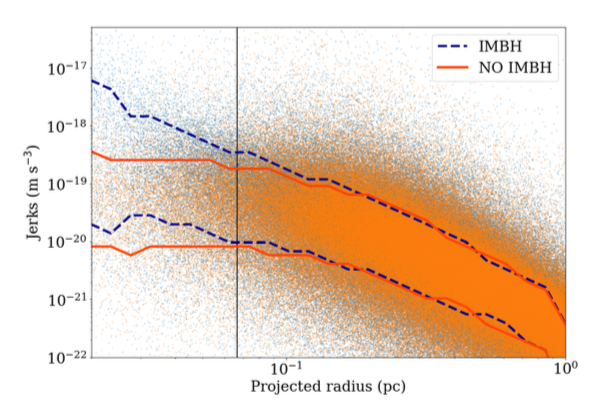
\includegraphics[width=0.6\columnwidth]{images/jerk_rad.png}
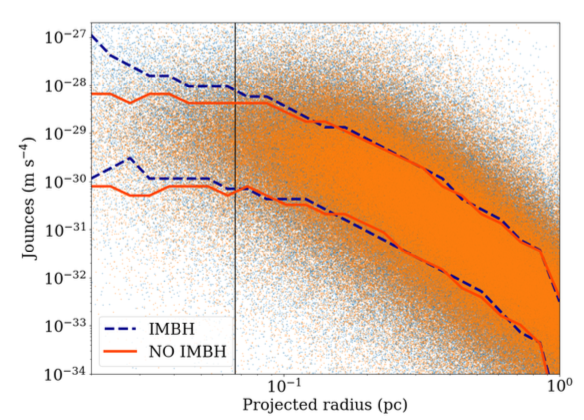
\includegraphics[width=0.6\columnwidth]{images/snap_rad.png}
\end{center}
\caption{Profili radiali di $jerk$ (in alto) e $snap$ (in basso) ottenuti dalle simulazioni di Abbate et al.2019.}
\label{fig:profili}
\end{figure}

\chapter{Tecniche di Machine Learning interpretabile: alberi decisionali}
\label{chap:cap2}
In questo Capitolo, in seguito ad una rapida introduzione generale al \textit{Machine Learning}, viene presentata una delle tecniche di \textit{Machine Learning interpretabile} e cioè gli alberi decisionali.\\
Vengono descritti i concetti fondamentali necessari per costruire le strutture ad albero, i problemi più importanti che si possono incontrare durante questa fase ed i metodi che si utilizzano per risolverli.\\
 In particolare, viene descritto l'algoritmo CART \cite{brei:book}, ovvero l'algoritmo utilizzato in questo lavoro, ed i metodi su cui esso si basa.

\section{Introduzione al Machine Learning}
\label{sec:ml}
Il \textit{Machine Learning, (ML)} è una branca dell’Intelligenza Artificiale e si pone l’obiettivo di far apprendere in modo automatico alle macchine attività svolte da noi esseri umani.\\
Più precisamente, si dice che un programma impara da una certa esperienza $E$ rispetto ad una classe di compiti $T$ ottenendo una \textit{performance P}, se la sua \textit{performance P} nel realizzare i compiti $T$, migliora con l’esperienza $E$ \cite{mitch:book}.\\
In altre parole, se un programma migliora lo svolgere di un \textit{task} rispetto a un’esperienza passata, si dice che ha imparato.\\
Questo avviene tramite l'apprendimento automatico. Esso può essere suddiviso in due importanti categorie: apprendimento supervisionato e apprendimento non supervisionato. 

 Gli algoritmi di apprendimento automatico supervisionato sono sequenze di operazioni che utilizzano i dati di allenamento (\textit{training set}) ricevuti in input per produrre un modello capace di risolvere un problema di classificazione o di regressione su dati di test (\textit{test set}) mai visti in precedenza, con una \textit{performance} che aumenta in funzione della quantità di dati di allenamento ricevuti. In primo luogo, quindi, l'algoritmo lavora su un sottoinsieme del \textit{dataset} chiamato \textit{training set}. Una volta costruito il modello, questo poi viene utilizzato per riconoscere e analizzare dati mai visti (chiamati dati del \textit{test set}).\\
Durante l'apprendimento supervisionato si hanno a disposizione sia i dati di input ($X$, matrice delle $features$ composta dalle variabili indipendenti che usiamo per la predizione), sia i dati di output ($Y$, composto dalle variabili dipendente che vogliamo predire chiamate $labels$). In questo caso si utilizza un algoritmo che apprende la funzione $f$ che dall’input genera l’output: $Y= f(X)$.\\
L’obiettivo è approssimare la funzione in modo che quando si ha un nuovo dato di input l’algoritmo sia in grado di prevedere il valore di output generato per quel dato.\\
I problemi di apprendimento supervisionato possono essere distinti in:
\begin{itemize}
    \item Classificazione: si tratta di un problema discreto, cioè la $label$ è una variabile categorica (si/no, vero/falso, 0/1/2…). Ad esempio, in campo medico, si potrebbe voler determinare in base ai risultati quantitativi di una biopsia se un caso di tumore è benigno o maligno;
    \item Regressione: si tratta di un problema continuo, cioè la $label$ è una variabile numerica. Ad esempio, il prezzo più probabile di una casa che si vuole prevedere sulla base dei metri quadri e della zona di interesse.   
\end{itemize}
Nell’apprendimento non supervisionato, invece, si ha solo la variabile di input $X$ e nessuna variabile di output corrispondente. Pertanto, gli algoritmi di apprendimento non supervisionato cercano di trovare una struttura nel $dataset$.\\
In questo caso i problemi di apprendimento possono essere suddivisi in:
\begin{itemize}
    \item Raggruppamento: anche detto \textit{clustering}, viene utilizzato quando è necessario raggruppare i dati che presentano caratteristiche simili. Per esempio un assicuratore potrebbe voler individuare clienti che corrispondono a profili di rischio simili tra loro, sulla base di caratteristiche quali: l'età, il genere, indicatori dello stato di salute, ecc...;
    \item Associazione: è un problema dove si vogliono scoprire regole che descrivono grandi porzioni di dati; si ha come obiettivo quello di trovare schemi frequenti, associazioni, correlazioni o strutture casuali tra un insieme di oggetti in un \textit{dataset} relazionale. Un'applicazione è quella del \textit{market basket analysis}. Si tratta di analisi di transazioni commerciali che possono produrre informazioni per determinare regole ricorrenti che pongono in relazione l’acquisto di uno o più prodotti con altri. Ad esempio, se un cliente compra il latte qual è la probabilità che compri anche i cereali? Sulla base di queste informazioni si possono progettare azioni promozionali o posizionare gli articoli sugli scaffali;
    \item Riduzione della dimensionalità: è un problema in cui si vuole individuare un numero ridotto di \textit{features} rappresentative delle caratteristiche dei dati all'interno di un grande campione di \textit{features} inizialmente disponibile. Ad esempio, uno psicologo potrebbe utilizzare dati di un campione di studenti delle scuole superiori per costruire un indicatore di abilità linguistica e uno di abilità numerica combinando i voti ricevuti nelle varie materie. Questo consentirebbe la visualizzazione di una pagella come un punto nel piano definito da queste due variabili, invece di trovarsi ad affrontare il problema più complesso di visualizzare contemporaneamente i voti di tutte le materie.
\end{itemize}

In questo lavoro di tesi ho utilizzato un metodo supervisionato  di classificazione: gli alberi decisionali. \MP{Qui direi perchè: sono intepretabili, che é il punto cardine della tesi} Nelle prossime Sezioni, infatti, saranno approfonditi gli aspetti teorici che li riguardano. 

\section{Concetti preliminari: notazione e struttura del dataset}
\label{sec:dataset_class}

In questa Sezione vengono esposti alcuni concetti preliminari che riguardano gli algoritmi di classificazione, necessari per entrare nel merito dei metodi utilizzati per questo lavoro.\\
Il $dataset$ sul quale avviene la fase di addestramento viene chiamato \textit{training set} e il modo più semplice per descriverlo è mediante una matrice $\mathbf{X} \in \mathbb{R}^{n \times \mathbf{m}}$. Le righe della matrice sono i $records$, ovvero gli esempi o le osservazioni e le colonne sono le $features$, cioè le caratteristiche multiple aventi per ogni esempio.\\
Per un algoritmo di classificazione, essendo un metodo di addestramento supervisionato, il $dataset$ è caratterizzato anche dal vettore $Y$ delle $labels$. Ogni $label$, ovvero ogni etichetta, corrisponde ad una classe e sono le variabili target che si vogliono predire (tab. \ref{tab:dataset}).\\

\begin{table}[ht]
    \centering
\begin{tabular}{|c|c|c|c|c|c|}
\hline & feat. $1\left(A_{1}\right)$ & feat. $2\left(A_{2}\right)$ & $\ldots \ldots \ldots$ & feat. $\mathrm{m}\left(A_{m}\right)$ & classe \\
\hline record 1 & & & & & \\
\hline record 2 & & & & & \\
\hline record 3 & & & & & \\
\hline$\ldots \ldots .$ & & & & & \\
\hline$\ldots \ldots$ & & & & & \\
\hline record n & & & & & \\
\hline
\end{tabular}
\caption{Schema della struttura di un generico $dataset$ di apprendimento nel caso in cui si stiano usando algoritmi di classificazione.}
\label{tab:dataset}
\end{table}

La classificazione ha come scopo quello di analizzare i dati di input sviluppando un modello in grado di predire la classe di appartenenza dei  \textit{records} in base alle \textit{features} presenti nei dati. In genere, partendo dall’utilizzo di insiemi esistenti e già classificati, l'algoritmo cerca di identificare alcune regolarità che caratterizzano le varie classi. 

\section{Alberi decisionali: concetti generali}
Gli alberi decisionali sono strutture molto conosciute nell'ambito degli algoritmi supervisionati, in quanto permettono di classificare in modo semplice degli oggetti in un numero finito di classi.

L'utilizzo degli alberi decisionali offre numerosi vantaggi:
\begin{itemize}
    \item sono di facile interpretazione, specie se non sono molto profondi;
    \item ottengono una buona accuratezza su gran parte dei problemi reali di classificazione su dati tabulari;
    \item sono robusti rispetto al rumore e alla ridondanza tra le \textit{features};
    \item possono essere costruiti efficientemente ed essere visualizzati.
\end{itemize}

Gli alberi vengono costruiti suddividendo i $records$ in sottoinsiemi in base alle relazioni che legano le variabili target, che si cercano di prevedere, alle \textit{features} utilizzate come predittori. In particolare, questo permette di costruire un modello rappresentato da un insieme di regole ottenute ponendo una serie di domande (test). Queste sono mirate sui valori delle \textit{features} e tipicamente consistenti in un confronto tra il valore di una data \textit{feature} e una soglia numerica. Ogni volta che si riceve una risposta viene posta la domanda successiva in modo che sia attinente al risultato ottenuto. Il processo viene iterato fino all'ottenimento della classe di ciascun $record$. La serie di domande, e le relative risposte sono organizzate in una struttura ad albero.\\
Fondamentalmente si tratta di una struttura semplice composta da nodi, rami e foglie (anche dette nodi terminali) che si sviluppa a partire dal nodo radice. Ogni nodo corrisponde ad una decisione basata sul confronto di una \textit{feature} con una costante. Essi sono collegati dai rami che identificano i livelli di parentela tra i diversi nodi (il nodo genitore rappresenta una decisione presa a monte rispetto al nodo figlio) e che forniscono gli strumenti per la costruzione di regole necessarie per classificare un oggetto. Infine, i risultati sono identificati dalle foglie. Dato un albero decisionale si possono ottenere predizioni rispetto a nuovi dati semplicemente percorrendo l'albero dalla radice verso le foglie, seguendo di volta in volta il ramo corrispondente al risultato del confronto effettuato in ciascun nodo.

Per fare maggiore chiarezza su come si costruisce un albero decisionale e sulla sua struttura, di seguito viene riportato un semplice esempio.\\
Supponiamo che una compagnia di assicurazioni voglia identificare il legame che lega le classi di rischio, in cui vengono suddivisi i clienti, con la loro età anagrafica e il tipo di vettura posseduto. Lo studio si deve basare su un gruppo di clienti già classificati nella corrispettiva classe.\\ 
Il \textit{training set} $T$ a disposizione è rappresentato in tabella \ref{tab:esempio} e l’insieme delle classi è $\Gamma = \{A, B\}$, in cui $A$ identifica un Alto rischio e $B$ un Basso rischio.

\begin{table}[ht]
    \centering
\begin{tabular}{|c|c|c|c|}
\hline Rid & Età & Tipo di Auto & Rischio \\
\hline 1 & 23 & Berlina & A \\
\hline 2 & 18 & Sportiva & A \\
\hline 3 & 43 & Sportiva & A \\
\hline 4 & 68 & Berlina & B \\
\hline 5 & 32 & Furgone & B \\
\hline6 & 20 & Berlina & A \\
\hline
\end{tabular}
\caption{$Dataset$ d’esempio per classificare clienti di una compagnia di assicurazioni in opportune classi di rischio.}
    \label{tab:esempio}
\end{table}
In figura \ref{fig:esempio} viene riportato un possibile albero decisionale per l'esempio in questione. Si noti come i nodi interni corrispondano a test sulle $features$ e come i nodi foglia vengano etichettati con la classe di maggioranza per la rispettiva foglia.
\begin{figure}
\begin{center}
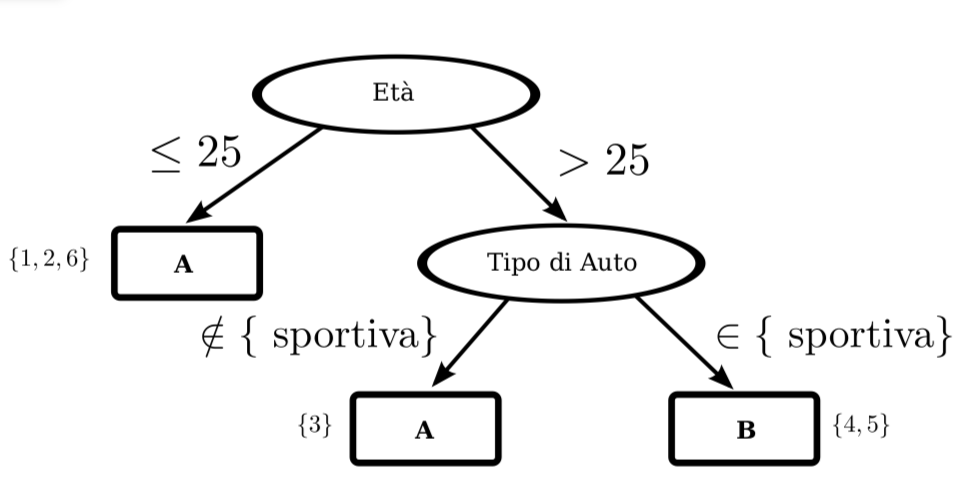
\includegraphics[width=0.5\columnwidth]{images/albero_esempio.png}
\end{center}
\caption{Esempio di albero decisionale per una compagnia di assicurazioni. \MP{Il labeling dell'ultimo nodo mi sembra sbagliato, sono quelli che hanno un'auto sportiva ($\in$ sportiva) che sono ad alto rischio nonostante siano vecchi; $A$ e $B$ nelle foglie andrebbero scambiati.}}
\label{fig:esempio}
\end{figure}

I test sulle \textit{features}, effettuati nei nodi interni, differiscono a seconda del tipo di dati. La suddivisione del $dataset$, dovuta ad esiti diversi nei test, è definita $split$.\\
In questo esempio gli $split$ sono binari, in quanto per ogni nodo si hanno a disposizione due possibilità.

\section{Algoritmo CART}
Esistono in letteratura diversi algoritmi di classificazione che fanno uso degli alberi decisionali. Quello che è stato utilizzato in questo lavoro è l'algoritmo CART.

L'algoritmo CART, \textit{Classification and Regression Trees} \cite{brei:book}, è uno degli algoritmi più conosciuti ed utilizzato per lo sviluppo di alberi decisionali e può lavorare sia come un classificatore che come un regressore.

Uno dei suoi punti di forza è la sua semplicità: esso opera mediante degli $split$ binari (ad ogni nodo corrispondono due soli rami) su una singola variabile in modo ricorsivo, quindi, classificare un campione può richiedere solo pochi semplici passi.\\
Nonostante la sua semplicità, è comunque in grado di ottenere risultati migliori di diversi altri metodi, su $dataset$ complessi, non lineari e composti da molte variabili.\\
Questo è senz'altro un valore aggiunto al fatto che gli alberi decisionali siano di così facile ed intuitiva interpretazione, per questo motivo vengono utilizzati negli ambiti più svariati. Quelle appena discusse sono anche le motivazioni primarie che hanno spinto all'utilizzo di tale metodologia per lo sviluppo di questo progetto di tesi. Trattandosi di un \textit{dataset} non ancora mai sottoposto ad uno studio con metodi di ML, gli alberi decisionali con l'algoritmo CART hanno fornito una prima analisi esplorativa dei dati fornendo già dei buoni risultati \ref{chap:cap4}.

Il metodo CART è molto efficiente anche perché non richiede in ambito applicativo di sperimentare trasformazioni delle variabili indipendenti (logaritmi, radici
quadrate, elevamento a potenza, ecc). Tali trasformazioni, in quanto monotóne, non modificano i risultati a meno che lo $split$ sia basato su combinazioni lineari delle variabili. Questo in genere non succede in un albero convenzionale, dove le \textit{features} vengono valutate indipendentemente in ciascun nodo. Inoltre, esso può utilizzare la stessa variabile in punti differenti dell’albero.\\ 
Il CART è stato creato con lo scopo di trattare dati dotati di una struttura complessa. E' estremamente robusto all’effetto degli \textit{outliers} e può utilizzare congiuntamente variabili di tipo categorico e continue.\\
L'algoritmo CART produce alberi ottimali, utilizzando strumenti sofisticati per stabilirne l'accuratezza (Sez.\ref{sec:metriche}). E, infine, oltre ad essere alla base di altri algoritmi che generano alberi più complessi, esso può essere utilizzato a supporto di altri tipi di modelli.

L'algoritmo si sviluppa in due fasi:
\begin{itemize}
    \item Fase di generazione dell'albero; 
    \item Fase di riduzione della complessità.
\end{itemize}
Vedremo ora quali sono in generale i criteri per la costruzione di alberi decisionali e su quali in particolare il CART si basa.

\section{Criteri per la costruzione di alberi decisionali}
Per costruire una struttura ad albero efficace occorre seguire tre $step$:
\begin{itemize}
    \item Selezionare una regola per lo $split$ per ogni nodo, ciò significa determinare le variabili indipendenti ed i rispettivi valori soglia, che saranno usati per partizionare il \textit{training set};
    \item Determinare quali nodi sono terminali, quindi decidere quando "fermarsi";
    \item Assegnare una classe ad ogni nodo terminale.
\end{itemize}

\section{Regole di Splitting}
Definire le regole di $splitting$ vuol dire identificare, per ogni nodo, una variabile sulla quale effettuare il test sulla base del rispettivo valore soglia utilizzato per il partizionamento del \textit{training set}.\\
Il punto è quello di scegliere in ogni nodo la migliore variabile di $split$, che garantisca la suddivisione dei $records$ presenti nel nodo in sottogruppi il più possibili omogenei al loro interno ed eterogenei tra loro in termini dei valori delle rispettive \textit{labels}.\\
Occorre, quindi, effettuare una sorta di valutazione della bontà degli $split$.\\
A tal proposito gli autori dell'algoritmo CART hanno sviluppato un $framework$ metodologico, introducendo il concetto generico di \textit{impurità}.\\
Intuitivamente, quando dividiamo i dati, vorremmo che la regione corrispondente a ciascun nodo foglia sia "pura", ovvero che la maggior parte dei dati in questa regione provenga dalla stessa classe e quindi che ci sia una classe dominante.

Consideriamo il seguente esempio \cite{split:online} mostrato in figura \ref{fig:impurità}. 
\begin{figure}[ht]
\begin{center}
\includegraphics[width=0.37\columnwidth]{images/impurità1.png}
\includegraphics[width=0.37\columnwidth]{images/impurità2.png}
\end{center}
\caption{Un semplice esempio di $splitting$. La figura a sinistra mostra il primo $split$ (linea blu), mentre quella a destra mostra anche il secondo (linea rossa).}
\label{fig:impurità}
\end{figure}
Qui abbiamo due classi: la classe \textbf{x} e la classe \textbf{o}. Le variabili di input sono la variabile orizzontale e quella verticale. Il primo $split$ viene fatto controllando se la variabile orizzontale è al di sopra o al di sotto di una soglia (la divisione è indicata dalla linea blu).\\
Potremmo considerare questo $split$ una buona divisione perché il lato sinistro è quasi puro in quanto la maggior parte dei punti appartiene alla classe \textbf{x} e solo due punti appartengono alla classe \textbf{o}. Il viceversa vale per il lato destro.\\
Proseguendo ad un livello più in basso nell'albero, vediamo che sono state create altre due divisioni (linee rosse). La regione in alto a sinistra (o il nodo foglia) contiene solo la classe \textbf{x}, così come quella in alto a destra. Invece le regioni in basso a sinistra ed in basso a destra contengono solo la classe \textbf{o}.\\
A questo punto non è necessario effettuare altri $split$ perché tutte le foglie sono pure al $100\%$.


\subsection{La funzione di impurità}
\label{subsec:impurita}
La misura di impurità può essere ricavata a partire dalla cosidetta funzione di impurità $\phi$.\\
Essa misura l'entità della purezza di una regione contenente osservazioni appartenenti a classi possibilmente diverse.

Supponiamo che il numero di classi sia $k$. Quindi la funzione di impurità è definita sul set di \textit{k-tuple} $p_{1},p_{2},...,p_{k}$, che sono le probabilità di ogni osservazione di appartenere ad una certa classe. Vale che $p_{j} \in[0,1]$ $\forall$  $j=1,...,k$ e $\sum_{j} p_{j}=1$.\\
Durante l'addestramento non si conoscono le reali probabilità; si utilizzano, infatti, le percentuali di osservazioni in classe 1, classe 2, classe 3 e così via, in base al set di dati di addestramento.\\
La funzione di impurità può essere pensata come una funzione avente valori tra 0 e 1 che fornisce una misura di quanto le osservazioni siano correttamente distribuite nelle classi.

Si definisce, per un generico nodo $t$, la misura di \textit{impurità} $i(t)$ come segue:
\begin{equation}
i(t)=\phi(p(1 \mid t), p(2 \mid t), \ldots, p(k \mid t))
\label{eq:impurity}
\end{equation}
ove $p(j \mid t)$, con $j=1,...,k$, è la probabilità stimata a posteriori di ottenere la classe $j$ per un'osservazione nel nodo $t$.\\
L’impurità di un nodo è massima quando tutte le classi sono presenti nella stessa proporzione, mentre è minima quando il nodo contiene casi appartenenti ad un’unica classe. La misura di impurità viene usata per decidere quale $split$ fare in un dato nodo, determinando in sostanza in che modo si fa crescere l'albero.

Misure di impurità più comuni sono:
\begin{itemize}
    \item L'indice di eterogeneità di Gini: $\operatorname{Gini}(t)=1-\sum_{j} p_{j}^{2}(t)$
    \item L'entropia: $H(t)=-\sum_{j} p_{j} \log _{2} p_{j}(t)$
    \item Il tasso di errata classificazione: $\operatorname{r}(t)=1-\max \left\{p_{j}(t): 1 \leq j \leq k \right\}$
\end{itemize}


Generalmente, in particolare negli algoritmi che lavorano con $splitting$ binari come CART, viene utilizzato l'indice di Gini.\\
Tale misura può essere interpretata come la stima della probabilità che un’osservazione scelta casualmente nel nodo $t$ sia assegnata alla classe errata.\\
Essa tende a dare luogo a suddivisioni bilanciate dal punto di vista del numero di casi inviati dallo $split$ nei due nodi figli, ovvero tende ad evitare i cosiddetti \textit{small splits}.

\section{Dichiarazione dei nodi terminali}
A questo punto, per completare la costruzione dell'albero è necessario passare per gli ultimi due $step$.\\ 
Bisogna capire, in primo luogo, quando arrestare la "crescita" dell'albero e quindi identificare i nodi terminali. Infine è necessario assegnare una classe ad ogni nodo terminale.  

\subsection{Criteri di arresto}
Nella maggior parte dei casi, se si lasciasse sviluppare un albero fino alle foglie estreme, si avrebbe una struttura molto grande e caratterizzata dal concatenarsi di numerose condizioni. Così facendo, il vantaggio della semplicità interpretativa, caratteristica degli alberi decisionali, verrebbe perso e si andrebbe incontro al problema dell'\textit{overfitting} (approfindito nella Sezione \ref{sec:overfitting}).\\
La dimensione eccessiva sarebbe dovuta al numero di nodi terminali o, equivalentemente, al numero di suddivisioni che essi rappresentano. Per questa ragione, per ovviare al problema, si può decidere di interrompere l’espansione dell’albero sulla base di determinati criteri.\\
Alcuni criteri comuni sono:
\begin{itemize}
    \item  continuare la crescita finché si raggiunge una certa profondità predefinita;
    \item continuare finché il numero di osservazioni in ciascun nodo terminale non superi una certa soglia;
    \item continuare finché tutti i nodi terminali non sono puri, cioè contengono solo una classe \MP{Questo è un po' come non fermarsi però}.
\end{itemize}

Queste soglie vanno decise a priori e influenzano direttamente la dimensione
dell’albero. Per questo motivo, sebbene sia questo il metodo più semplice,
risulta piuttosto inefficiente perché rischia di sfoltire l'albero troppo o troppo poco rispetto al necessario, in base a quanto sia restrittivo il criterio d’arresto.

\subsection{Assegnazione della classe al nodo terminale}
Nella fase di assegnazione di una delle classi ai nodi terminali si possono
presentare tre situazioni diverse:
\begin{itemize}
    \item il nodo contiene solo osservazioni appartenenti alla stessa classe;
    \item il nodo contiene osservazioni appartenenti a classi diverse, ma una di queste presenta una proporzione di osservazioni maggiore delle altre;
    \item Il nodo contiene osservazioni appartenenti a classi diverse e nella stessa proporzione.
\end{itemize}
Nel primo caso l’assegnazione viene effettuata precisamente senza alcun tipo di
indecisione e nel secondo caso il nodo viene assegnato alla classe che presenta più osservazioni. Nell'ultimo caso, invece, si presenta una situazione di massima incertezza, in quanto la probabilità delle classi risulta identica per ciascuna di esse. Pertanto si ricorre ad un tipo di assegnazione
casuale salvo l'intervento del ricercatore che può effettuare un’assegnazione diversa sulla base delle sue conoscenze.

\section{Problema dell'overfitting}
\label{sec:overfitting}
Alla fase di costruzione dell'albero decisionale, per far sì che esso si comporti come un buon classificatore, segue la fase di riduzione della complessità dell'albero. Ma prima di approfondire la descrizione che riguarda questa seconda fase, bisogna introdurre un problema con il quale, quasi sempre, tutti gli algoritmi di ML si confrontano: il problema dell'\textit{overfitting}.

Il metodo di classificazione è un processo che si sviluppa in due fasi: la fase di apprendimento e la fase di predizione.\\ 
Nella fase di apprendimento, il modello viene sviluppato sulla base di dati di allenamento conosciuti, che abbiamo chiamato \textit{training set}.\\
Successivamente, la fase di predizione viene eseguita su un insieme di dati totalmente nuovi per il modello, il cosiddetto \textit{test set}.\\
In pratica, quindi, il modello apprende informazioni, relazioni e collegamenti durante la prima fase e poi applica tutto ciò che ha acquisito su un nuovo insieme di dati per fornire una predizione.\\
Quello che normalmente accade \MP{dipende... se si allena un modello rigido, per es. una regressione lineare, questo non succede} nelle prime prove di addestramento è che il modello porta a delle prestazioni molto buone sul \textit{trainig set} e alquanto scadenti sul \textit{test set}. Vuol dire che il modello 'impara troppo bene' gli schemi dal \textit{training set}, così tanto da non essere poi in grado di generalizzare quanto appreso su un nuovo gruppo di dati.
\MP{Più che 'imparare troppo bene', il modello impara caratteristiche del training set che sono proprie solo del training set e non si applicano altrove. Per esempio nel training set, per puro caso, tutti i fumatori erano pisani. Nella realtà anche persone di altre città fumano con la stessa probabilità e quindi la città di provenienza è pressoché inutile per prevedere se una persona fuma o meno. Ma, specialmente in training set piccoli, correlazioni spurie di questo tipo possono verificarsi abbastanza di frequente.}

Per 'generalizzazione', quindi, si intende l’abilità di una macchina di portare a termine in maniera accurata esempi o compiti nuovi, che non ha mai affrontato, dopo aver fatto esperienza su un insieme di dati di apprendimento \cite{generalizz:online}.\\
Questo problema è noto con il termine \textit{overfitting}, ovvero si tratta di un problema di sovradattamento da parte del modello ai dati \textit{trainig set}. Si verifica quando il modello viene addestrato eccessivamente su un set di dati rumorosi.\\
Pertanto, a causa di questo problema, quando si sviluppa un albero decisionale, è importante capire quando fermarsi. Se un albero crescesse troppo, fino alle foglie più estreme, oltre a perdere la sua importante caratteristica di essere interpretabile, si andrebbe incontro al problema dell'\textit{overfitting}. Questo è evidente se, ad esempio, avessimo un albero con una sola osservazione per foglia, raggiungendo quindi una purezza perfetta in ciascuna foglia sul \textit{training set}. Se si estendesse al massimo un albero, infatti, tale obbiettivo si potrebbe sempre raggiungere per qualunque scelta dei dati di $training$, ma negli ultimi $split$ l'albero non avrebbe imparato alcuna informazione utile dai dati, adattandosi solo alle idiosincrasie del \textit{training set}. Pertanto, risulterebbe probabile che la \textit{performance} predittiva su dati non visti sia molto inferiore, nonostante la predizione nominalmente perfetta in $training$.

Una tecnica per risolvere tale problema per gli alberi decisionali è la tecnica del \textit{pruning}. In breve, essa consiste nell’ottenere da un albero il più piccolo “sottoalbero” che, di fatto, non comprometta l’accuratezza della classificazione. In particolare, nell'algoritmo CART, la tecnica utilizzata è quella del \textit{Cost-Complexity Pruning} che verrà approfondita nella prossima Sezione.

\section{Cost-Complexity Pruning}
\label{sec:pruning}
Per ridurre la complessità dell'albero affinchè possa essere effettivamente utile nel classificare $records$ e nel fornire regole efficaci, è necessario sfoltire la ridondanza dell’albero, ovvero eliminanare i rami meno significativi.

La tecnica che l'algoritmo CART utilizza prende il nome di \textit{Cost-Complexity Pruning}. Consiste nel far sviluppare l'intero albero e poi estarre da esso il più piccolo "sottoalbero". Quest'ultimo porterà a delle migliori previsioni perché vi sono stati "tagliati" i rami corrispondenti a \textit{splitting} eccessivamente specifici sul \textit{training set} e, quindi, superflui. Infatti \textit{pruning} sta proprio per "potatura".\\ 
Questo processo, appunto, non peggiora l'accuratezza delle previsioni, ma bensì, in genere, le migliora, in quanto, poi, il modello sarà capace di classificare efficientemente anche dati totalmente nuovi.

\subsection{Notazione e metodo}
Ora viene introdotta la notazione necessaria per la trattazione della tecnica del \textit{Cost-Complexity Pruning}.\\
Si definiscono:
\begin{itemize}
    \item $T_{max}$ dimensione di massima crescita dell'albero $T$;
    \item $t$ i nodi genitori;
    \item $t'$ i nodi figli, cioè un nodo collegato tramite un percorso al nodo $t$;
    \item $T_{t}$ un ramo dell'albero $T$ con nodo radice $t$.
\end{itemize}
Un metodo di potatura efficiente dovrebbe garantire che la ricerca della sottostruttura ottimale possa essere trattabile computazionalmente.

L'algoritmo del \textit{Cost-Complexity Pruning} è parametrizzato dal parametro $\alpha \in \mathbb{R}$, $\alpha \in[0,1]$, noto come \textit{parametro di complessità}. Questo parametro viene utilizzato per definire la misura \textit{cost-complexity} $R_{\alpha}(T)$ per ogni sottostruttura $T<T_{max}$ come:
\begin{equation}
R_{\alpha}(T)=R(T)+\alpha|\tilde{T}|
\label{eq:costcompl}
\end{equation}
dove $R(T)$ è il tasso di errata classificazione totale dei nodi terminali (definito \ref{subsec:impurita}) e $|\tilde{T}|$ è il numero di nodi terminali (o nodi foglia) che definisce la complessità dell'albero $T$. Infatti, maggiore è il numero di nodi foglia che l'albero contiene, maggiore è la complessità dell'albero perché vi è maggiore flessibilità nel partizionare lo spazio in parti più piccole e quindi maggiori possibilità di adattare i dati di addestramento.\\
Durante la potatura dell'abero bisogna minimizzare la funzione $R_{\alpha}(T)$ e la sottostruttura che alla fine verrà selezionata dipende dal parametro $\alpha$. Infatti, se $\alpha=0$ verrà scelto l'albero più grande perché il termine di complessità viene essenzialmente eliminato. Per $\alpha$ tendente all'infinito, invece, verrà selezionato l'albero di dimensione 1, cioè un singolo nodo radice.\\
Si può dimostrare \cite{split:online} che per ogni $\alpha$ esiste ed è unica una sottostruttura che minimizza $R_{\alpha}(T)$. Inoltre, si può dimostrare anche che le sottostrutture che minimizzano $R_{\alpha}(T)$ al crescere di $\alpha$ sono annidate. Ovvero, il sottoalbero dell'$\alpha$ successivo è compreso in quello precedente e, quindi, vale che $T_{1}>T_{2}>\cdots>t_{1}$, dove i pedici rappresentano il numero progressivo degli $\alpha$. Praticamente, a partire dalle foglie l'algoritmo procede spostandosi verso la radice valutando in ogni nodo la \textit{cost-complexity} al variare di $\alpha$.

Per fare maggiore chiarezza sul metodo di taglio, in primo luogo, è necessario estendere la definizione \ref{eq:costcompl} a un nodo e ad un singolo ramo fuoriuscente dal nodo:
\begin{itemize}
    \item per qualsiasi nodo $t$ appartenente ad una sottostruttura la \ref{eq:costcompl} diventa: $$R_{\alpha}(t)=R(t)+\alpha$$in quanto ci si sta riferendo proprio ad un nodo, in questo caso non c'è il termine di complessità $|\tilde{T}|$ \MP{non è che non ci sia, ma è uguale a $1$};  
    \item per qualsiasi ramo $T_{t}$, invece la \ref{eq:costcompl} diventa: $$R_{\alpha}\left(T_{t}\right)=R\left(T_{t}\right)+\alpha\left|\tilde{T}_{t}\right|$$ in cui il termine $R\left(T_{t}\right)$ è calcolato considerando tutti i nodi terminali che discendono dal nodo $t$ attraverso il ramo $T_{t}$ (Fig. \ref{fig:potatura}).
\end{itemize}
In ogni nodo, facendo variare $\alpha$ tra 0 e 1 in maniera crescente, l'algoritmo confronta il \textit{cost-complexity} calcolato nel nodo $t$ con quello calcolato per il ramo $T_{t}$. Affinchè l'algoritmo decida di non tagliare un ramo, lo $split$ che avviene per mezzo di esso, deve essere efficiente. Questo si verifica quando lo $split$ riduce l'errore sulla classificazione. Pertanto, finchè $R_{\alpha}\left(T_{t}\right)<R_{\alpha}(t)$ il ramo viene tenuto, ma nonappena i due valori si eguagliano esso viene tagliato. Per cui, la condizione di taglio è data da $R_{\alpha}\left(T_{t}\right)=R_{\alpha}(t)$, da cui:
\begin{equation}
\alpha=\frac{R(t)-R\left(T_{t}\right)}{\left|\tilde{T}_{t}\right|-1}
\label{eq:taglio}
\end{equation}
L'algoritmo lavora percorrendo a ritroso l'albero, dalle foglie verso la radice.\\ Inizialmente, quindi, considera tutti i nodi che precedono le foglie e, facendo variare $\alpha$, il primo nodo trovato che soddisfa la condizione \ref{eq:taglio} viene tagliato. A questo punto, l'algoritmo salva in memoria l'$\alpha$ appena ricavato e poi procede al passo successivo considerando l'albero appena ottenuto come albero iniziale. 
\begin{figure}
\begin{center}
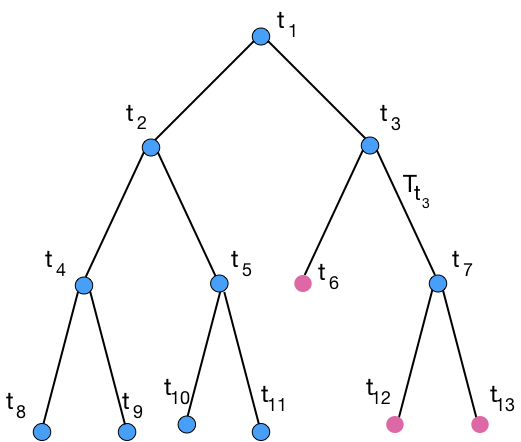
\includegraphics[width=0.37\columnwidth]{images/albero1.png}
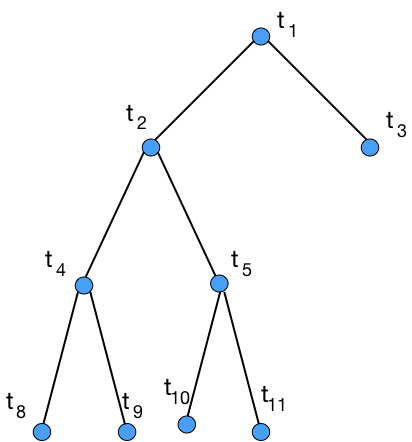
\includegraphics[width=0.30\columnwidth]{images/albero2.png}
\end{center}
\caption{Un semplice schema di una struttura ad albero. I nodi terminali del ramo $T_{t_{3}}$ sono $t_{6}$, $t_{12}$ e $t_{13}$ (a sinistra). In $t_{3}$ si verifica la condizione \ref{eq:taglio}, per cui l'intero ramo $T_{t_{3}}$ viene tagliato (a destra).}
\label{fig:potatura}
\end{figure}

\MP{nella sezione appena conclusa sottolineerei che $\alpha$ è un parametro che l'utente sceglie a mano e che quindi va determinato in base a conoscenze specifiche legate al problema oppure sperimentalmente, tramite validation. Così si transisce in modo naturale alla prossima sezione.}

\section{Training, validation e test sets}
\label{sec:splitdata}
Per identificare i parametri da fornire ai modelli di ML è di uso comune suddividere il \textit{dataset} in tre sottogruppi: \textit{training set, validation set} e \textit{test set}.\\
In questo caso particolare, per effettuare un \textit{pruning} efficiente, dal punto di vista pratico, è necessario identificare il parametro di complessità $\alpha$ al quale corrisponderebbe la miglior sottostruttura dell'albero $T$. Infatti, come spiegato nel paragrafo precedente, ad ogni passo l'algoritmo \textit{Cost-Complexity Pruning} salva in memoria il parametro $\alpha$ che soddisfa la relazione \ref{eq:taglio} con il relativo modello ad albero. Sarà l'utente, in una fase successiva, a scegliere tra questi la miglior sottostruttura, cioè quella per cui si ottiene la miglior accuratezza nella classificazione. Per questo motivo si divide il \textit{dataset} in tre sottogruppi.

Il \textit{training set} è l'insieme di dati con i $records$ e le relative $labels$ e serve al classificatore durante la fasse di allenamento per apprendere gli schemi che possono essere utilizzati successivamente per prevedere le $labels$ dei nuovi dati. In questa fase è importante che non venga effettuata nessuna scelta sul modello.

Il \textit{validation set}, invece, è utile per determinare con quali parametri l'algoritmo di classifcazione avrebbe le migliori prestazioni. Nel caso degli alberi decisionali la fase di validazione è necessaria per scegliere il miglior parametro di complessità $\alpha$.

Una volta ottenuto il miglior classificatore bisogna valutare le sue prestazioni su un set di dati completamente nuovo per lui: il \textit{test set}.

La scelta su come effettuare la divisione del \textit{dataset} è individuale, ma generalmente il \textit{test set} rappresenta circa il $20-30\%$ dei dati. La restante parte del \textit{dataset} viene suddiviso nel seguente modo: circa il $70-80\%$ dei dati rimasti costituirà il \textit{training set} e circa il $20-30\%$ farà parte del \textit{validation set}. 

\begin{figure}
\begin{center}
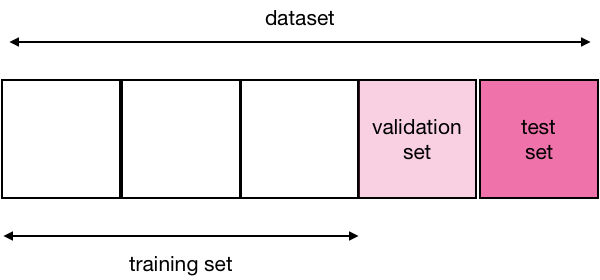
\includegraphics[width=0.6\columnwidth]{images/dataset.png}
\end{center}
\caption{Schema per visualizzare la divisione dei dati nei tre sottogruppi: \textit{training set, validation set} e \textit{test set}.}
\label{fig:dataset}
\end{figure}

\section{Qualità delle previsioni}
\label{sec:metriche}
Per qualsiasi algoritmo di ML, dopo aver ottenuto le previsioni, bisogna valutarne la qualità. Per quantificare la bontà delle \textit{performance} possono essere utilizzate diverse metriche.\\
In questo lavoro, per valutare le prestazioni della classificazione da parte degli alberi decisionali, in primo luogo, è stata utilizzata l'\textit{accuratezza} e, successivamente, altre metriche più adatte \MP{in che senso? Avevamo notato che la sola acciratezza su un dataset sbilanciato dava risultati pessimi, ma poi hai bilanciato il dataset... direi semplicemente altre metriche, che misurano aspetti specifici delle prestazioni di classificazione}, come \textit{precisione, richiamo} ed \textit{F-score (o F-1)}. \MP{Peraltro poi queste metriche vanno spiegate bene, se non qui nel seguito (nel qual caso indicherei che esse sono spiegate nel seguito).}

\subsection{Accuratezza degli alberi decisionali}
Per definire l'accuratezza di un albero decisionale, in primo luogo, introduciamo una notazione. Indichiamo con:
\begin{itemize}
    \item $\bar{n}_{t}$ il numero totale dei $records$ del \textit{test set} che finiscono nel nodo terminale $t$;
    \item $n_{t}$ il numero di $records$ classificati correttamente in $t$.
\end{itemize}
Ad ogni nodo terminale $t$ è possibile associare un'accuratezza $a_{t}$ data dalla frazione dei $records$ classificati correttamente nella data foglia $t$:
\begin{equation}
a_{t}=\frac{n_{t}}{\bar{n}_{t}}
\label{eq:acc_t}
\end{equation}
L’accuratezza nella classificazione associato all’intero albero è data dalla somma delle accuratezze calcolate su tutti i $t$, pesate rispetto alla probabilità che un $record$ possa finire su ciascuna foglia.\\
Se il numero totale di $records$ è $N$ , allora, la probabilità che un certo $record$ finisca nella foglia $t$ è data da $\frac{\bar{n}_{i}}{N}$. Pertanto l'accuratezza $A$ dell'albero risulta:
\begin{equation}
A=\sum_{t} \frac{\bar{n}_{t}}{N} a_{t}
\label{eq:acc}
\end{equation}
La situazione ideale si ha quando $A=1$, in cui il modello è in grado di classificare perfettamente tutti i $records$.\\ 
Questa metrica di solito lavora bene su un set di dati bilanciato, ovvero quando si ha un numero simile di campioni appartenenti a ogni classe.\\
L'accuratezza, però, non è il miglior metodo per valutare le prestazioni di un classificatore.

\subsection{Matrice di confusione: precisione, richiamo e F-score}
\label{subsec:confmatr}
Uno strumento intuitivo per valutare le \textit{performance} di un modello di classificazione è la \textit{matrice di confusione}. Per analizzare le informazioni che essa fornisce bisogna definire le metriche che utilizza e cioè la \textit{precisione}, il \textit{richiamo} e la \textit{F-score (o F-1)}.

Supponiamo di avere due classi: la classe $P$ dei positivi e la classe $N$ dei negativi.\\
Allora, le previsioni ottenute da un modello su un \textit{test set} possono essere definite nei seguenti modi:
\begin{itemize}
    \item \textbf{Veri Positivi} (TP), sono i dati test \MP{realmente} etichettati come $P$ e che il modello ha previsto correttamente come $P$;
    \item \textbf{Falsi Positivi} (FP), sono i dati test etichettati come $N$, ma per i quali il modello ha predetto essere $P$;
    \item \textbf{Falsi Negativi} (FN), sono i dati test appartenenti alla classe $P$, ma per cui il modello ha predetto come $N$;
    \item \textbf{Veri Negativi} (TN), sono i dati test della classe $N$ per i quali il modello ha predetto correttamente collocandoli nella classe $N$.
\end{itemize}
A partire da queste definizioni è possibile introdurre le metriche:
\begin{itemize}
    \item \textbf{Precisione}, $P=\frac{\mathrm{TP}}{T P+F P}$ \MP{il comando mathrm ti permette di far apparire il testo come testo normale dentro ad una espressione matematica; forse puoi provare a usarlo se ti piace il risultato}, è il numero di TP diviso per il numero di classificazioni positive, cioè TP e FP \MP{darei degli esempi: il numero di persone veramente malate su quelle che un dato test ritiene malate}; 
    \item \textbf{Richiamo}, $R=\frac{T P}{T P+F N}$, è il numero di TP diviso per il numero di tutti i $records$ positivi, cioè TP e FN \MP{il numero di persone malate individuate da un test sul totale delle persone veramente malate}; 
    \item \textbf{F-score}, $F_{1}=2 \cdot \frac{P \cdot R}{P+R}$, è una media armonica tra precisione e richiamo \MP{indicherei qui che la media armonica è più vicina al minimo di quanto lo sia la media aritmetica, quindi per ottenere una buona F score bisogna avere sia un buon richiamo che una buona precisione (come dici dopo)}.
\end{itemize}
Un valore vicino a 1 della \textit{F-score} segnala la capacità del modello di classificare correttamente la maggior parte dei dati, ottenendo sia una buona precisione che un buon richiamo (Fig. \ref{fig:prec_ric}). \MP{D'altra parte ottenere un buon richiamo con una pessima precisione è semplice: basta dichiarare tutti malati, riducendo così a zero il numero di falsi negativi al costo di avere molti falsi positivi. Ma il classificatore che ne risulta 
è inutile. Per questo il richiamo da solo non è una buona metrica. Per ragioni analoghe (potrei dichiarare che nessuno è malato, portando i falsi positivi a zero assieme ai veri positivi) la precisione da sola è a sua volta una metrica non buona. Combinandole, la F-score ci garantisce una misura più bilanciata tra questi due aspetti.}

\begin{figure}[ht]
\begin{center}
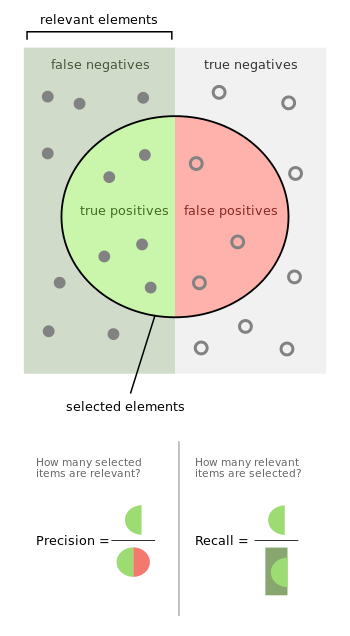
\includegraphics[width=0.4\columnwidth]{images/prec_ric.png}
\end{center}
\caption{Schematizzazione visiva di TP, FP, TN, FN e delle metriche di precisione e richiamo \cite{prec_ric:online}.}
\label{fig:prec_ric}
\end{figure}


Un metodo molto utile per visualizzare queste metriche è la matrice di confusione. Si tratta di uno strumento che mostra la frequenza di errori di classificazione e la corretta classificazione dei dati.\\
Nelle celle di una matrice di confusione sono riportati valori numerici per indicare i vari casi (TP, FP, TN e FN). Pertanto la precisione, il richiamo e, di conseguenza, l' \textit{F-score}, possono essere calcolati direttamente dai valori delle celle di una matrice di confusione.\\
In figura \ref{fig:conf_matr} è riportato uno schema d'esempio di matrice di confusione per un problema di classificazione con due classi.
\begin{figure}[ht]
\begin{center}

\includegraphics[width=0.5\columnwidth]{images/conf_matr_ok.png}
\end{center}
\caption{Struttura della matrice di confusione nel caso di un problema di classificazione con due classi: $P$ e $N$.}
\label{fig:conf_matr}
\end{figure}

\chapter{Alberi decisionali per l'identificazione di IMBHs}
\label{chap:cap3}
Dopo aver introdotto gli strumenti teorici necessari, in questo Capitolo viene descritta nello specifico l'applicazione di tali concetti al problema astrofisico in questione: l'identificazione di IMBHs al centro di GCs. In particolare, in questo lavoro di tesi, si vuole predire la presenza di IMBHs al centro dei GCs utilizzando un metodo di ML interpretabile sulla base delle caratteristiche dinamiche delle MSPs presenti nelle regioni centrali degli ammassi. I modelli di ML utilizzati sono gli alberi decisionali costruiti con l'algoritmo CART (Cap. \ref{chap:cap2}). 

In primo luogo verrà brevemente descritto il codice HiGPUs utilizzato per le simulazioni a N-corpi da cui provengono i \textit{dataset} forniti all'albero decisionale. Successivamente verranno, quindi, presentati i \textit{dataset} e poi si passerà ad una descrizione generale del codice sviluppato per la predizione.

\section{Motivazioni}
Nel Capitolo \ref{chap:cap1} si è parlato dell'importanza di identificare IMBHs al centro di ammassi e delle problematiche che si riscontrano utilizzando i metodi diretti. Abbiamo visto che esse sono legate principalmente alle difficoltà osservative, in quanto misurare le dispersioni di velocità all'interno della sfera di influenza del GC richiede elevatissime risoluzioni spaziali. Inoltre, l'identificazione di una cuspide nei profili di densità e di dispersione di velocità non sempre è indice della presenza di un IMBH.
Per lo sviluppo della tesi, invece, ci si è basati su un metodo di identificazione indiretto, ovvero quello delle MSPs \cite{abbate1:paper}. Dallo studio delle informazioni dinamiche delle MSPs all'interno dei GCs, infatti, è possibile identificare indirettamente la presenza di IMBHs in ammassi. 

In questo lavoro di tesi, però, si vuole applicare un nuovo metodo in questo contesto, ovvero servirsi di un algoritmo di ML interpretabile (gli alberi decisionali) per prevedere la presenza di IMBHs al centro di GCs. La sfida, infatti, sta proprio nel voler mettere a punto un metodo identificativo nuovo per cercare di avanzare nella risoluzione di un problema astrofisico ancora così aperto. Le informazioni delle MSPs che si vogliono fornire all'algoritmo per la predizione di IMBHs sono l'accelerazione e le sue derivate rispetto al tempo: \textit{jerks} e \textit{snaps (o jounce)}. Queste quantità sono legate alle derivate dei periodi delle MSPs nell'ammasso e, di conseguenza, sarebbe possibile stimarle a partire da tali misure. Le campagne osservative, tuttavia, richiedono tempistiche di diversi anni per ottenere \textit{jerks} e \textit{snaps} con una precisione adeguata, oltre a richiedere una certa regolarità e puntualità nelle osservazioni. Pertanto, i dati osservativi necessari non sono ancora a disposizione e, per questo lavoro, ci si è serviti dei dati provenienti da un set di simulazioni a N-corpi. Inoltre, avere dati di simulazioni in tal senso è di fondamentale importanza per un futuro confronto tra dati osservati e dati teorici. \MP{NB che il training va comunque fatto su simulazioni perché anche avendo dati di jerk e snap in ammassi reali non avremmo le etichette, visto che non sappiamo quali ammassi reali siano IMBH host e quali non lo siano.}

\section{HiGPUs}
Le simulazioni a N-corpi da cui derivano i dati forniti all'algoritmo di ML per la previsione di IMBHs nei GCs sono state ottenute mediante la nuova versione del codice \textit{HermiteIntegratorGPUs (HiGPUs)} \cite{capdolspe:paper}. Si tratta di un codice ad alta precisione, adatto a simulare l'evoluzione nel tempo di sistemi di masse puntiformi che interagiscono tramite la forza newtoniana classica.

Il codice HiGPUs (disponibile gratuitamente in \cite{HiGPUs:online}) implementa un metodo di integrazione di Hermite fino al $6^{\circ}$ordine e utilizza accelerazioni, \textit{jerks} e \textit{snaps} per far avanzare le posizioni e le velocità delle stelle nel tempo.

Lo schema che segue è diviso in tre fasi: predizione, valutazione e correzione. Di seguito verranno indicate le derivate dell'accelerazione rispetto al tempo con la notazione con i punti e chiameremo indistintamente gli elementi \textit{stelle} o \textit{particelle}. Consideriamo, quindi, un sistema composto da $N$ stelle e assumiamo che l'\textit{i-esima} particella al tempo iniziale $t_{c,0}$ sia caratterizzata da posizione $\textbf{r}_{i,0}$, velocità $\textbf{v}_{i,0}$, accelerazione $\textbf{a}_{i,0}$, \textit{jerk} $\dot{\mathbf{a}}_{i, 0}$, \textit{snap} $\ddot{\mathbf{a}}_{i, 0}$, \textit{crackle} $\dddot{\mathbf{a}}_{i, 0}$ ed un \textit{time step} $\Delta t_{i,0}$. Inoltre, chiamiamo $m$ il numero
di particelle appartenenti allo stesso blocco temporale e che devono essere evolute allo stesso tempo $t_{c,0} + \Delta t_{i,0}$. I passi da seguire sono, dunque, i seguenti:
\begin{itemize}
    \item \textit{Predizione}: consiste nel calcolo di posizione, velocità e accelerazione di tutte le stelle a partire dai valori iniziali:
    \begin{equation}
\begin{aligned}
\mathbf{r}_{i, p r e d} &=\mathbf{r}_{i, 0}+\mathbf{v}_{i, 0} \Delta t_{i, 0}+\frac{1}{2} \mathbf{a}_{i, 0} \Delta t_{i, 0}^{2}+\frac{1}{6} \dot{\mathbf{a}}_{i, 0} \Delta t_{i, 0}^{3}+\\
&+\frac{1}{24} \ddot{\mathbf{a}}_{i, 0} \Delta t_{i, 0}^{4}+\frac{1}{120} \dddot{\mathbf{a}}_{i, 0} \Delta t_{i, 0}^{5} \\
\mathbf{v}_{i, p r e d} &=\mathbf{v}_{i, 0}+\mathbf{a}_{i, 0} \Delta t_{i, 0}+\frac{1}{2} \dot{\mathbf{a}}_{i, 0} \Delta t_{i, 0}^{2}+\frac{1}{6} \ddot{\mathbf{a}}_{i, 0} \Delta t_{i, 0}^{3}+\\
&+\frac{1}{24} \dddot{\mathbf{a}}_{i, 0} \Delta t_{i, 0}^{4} \\
\mathbf{a}_{i, p r e d} &=\mathbf{a}_{i, 0}+\dot{\mathbf{a}}_{i, 0} \Delta t_{i, 0}+\frac{1}{2} \ddot{\mathbf{a}}_{i, 0} \Delta t_{i, 0}^{2}+\frac{1}{6} \dddot{\mathbf{a}}_{i, 0} \Delta t_{i, 0}^{3}
\end{aligned}
\label{eq:pred}
\end{equation}
    \item \textit{Valutazione}: calcolo dell'accelerazione e delle sue derivate prima e seconda per tutte le particelle $m<N$ sulla base delle posizioni e velocità predette. Le mutue interazioni tra l'\textit{i-esima} particella e le $N-1$ rimanenti sono descritte dalle seguenti relazioni:
    \begin{equation}
\begin{aligned}
\mathbf{a}_{i, 1}=& \sum_{j=1 \atop j \neq i}^{N} \mathbf{a}_{i j, 1}=\sum_{j=1 \atop j \neq i}^{N} m_{j} \frac{\mathbf{r}_{i j}}{r_{i j}^{3}} \\
\dot{\mathbf{a}}_{i, 1}=& \sum_{j=1 \atop j \neq i}^{N} \dot{\mathbf{a}}_{i j, 1}=\sum_{j=1 \atop j \neq i}^{N}\left(m_{j} \frac{\mathbf{v}_{i j}}{r_{i j}^{3}}-3 \alpha_{i j} \mathbf{a}_{i j, 1}\right) \\
\ddot{\mathbf{a}}_{i, 1}=& \sum_{j=1 \atop j \neq i}^{N} \ddot{\mathbf{a}}_{i j, 1}=\sum_{j=1 \atop j \neq i}^{N}\left(m_{j} \frac{\mathbf{a}_{i j}}{r_{i j}^{3}}-6 \alpha \dot{\mathbf{a}}_{i j, 1}-3 \beta_{i j} \mathbf{a}_{i j, 1}\right)
\end{aligned}
\label{eq:valut}
\end{equation}
dove $\mathbf{r}_{i j} \equiv \mathbf{r}_{j, p r e d}-\mathbf{r}_{i, \text {pred}}, \mathbf{v}_{i j} \equiv \mathbf{v}_{j, \text {pred}}-\mathbf{v}_{i, \text {pred}}, \mathbf{a}_{i j} \equiv \mathbf{a}_{j, \text {pred}}-\mathbf{a}_{i, \text {pred}},$
$\alpha_{i j} r_{i j}^{2} \equiv \mathbf{r}_{i j} \cdot \mathbf{v}_{i j}, \beta_{i j} r_{i j}^{2} \equiv v_{i j}^{2}+\mathbf{r}_{i j} \cdot \mathbf{a}_{i j}+\alpha_{i j}^{2} r_{i j}^{2}$
    \item \textit{Correzione}: le posizioni e le velocità delle $m$ particelle vengono corrette per mezzo delle accelerazioni e relative derivate secondo le relazioni:
    \begin{equation}
\begin{aligned}
\mathbf{v}_{i, \text {corr}} &=\mathbf{v}_{i, 0}+\frac{\Delta t_{i, 0}}{2}\left(\mathbf{a}_{i, 1}+\mathbf{a}_{i, 0}\right)-\frac{\Delta t_{i, 0}^{2}}{10}\left(\dot{\mathbf{a}}_{i, 1}-\dot{\mathbf{a}}_{i, 0}\right)+\\
&+\frac{\Delta t_{i, 0}^{3}}{120}\left(\ddot{\mathbf{a}}_{i, 1}+\ddot{\mathbf{a}}_{i, 0}\right) \\
\mathbf{r}_{i, c o r r} &=\mathbf{r}_{i, 0}+\frac{\Delta t_{i, 0}}{2}\left(\mathbf{v}_{i, \operatorname{corr}}+\mathbf{v}_{i, 0}\right)-\frac{\Delta t_{i, 0}^{2}}{10}\left(\mathbf{a}_{i, 1}-\mathbf{a}_{i, 0}\right)+\\
&+\frac{\Delta t_{i, 0}^{3}}{120}\left(\dot{\mathbf{a}}_{i, 1}+\dot{\mathbf{a}}_{i, 0}\right)
\end{aligned}
\label{eq:correz}
\end{equation}
\end{itemize}

HiGPUs è un codice ad alta precisione perché oltre ad utilizzare l'integrazione di Hermite fino al $6^{\circ}$ ordine, calcola sempre le interazioni mutue tra tutte le stelle e definisce un \textit{time step} variabile per ciascuna stella sulla base delle loro accelerazioni. Questo garantisce un buon compromesso tra precisione e velocità di calcolo. 

Tuttavia, utilizzando intervalli temporali differenti durante l’integrazione, nel caso di incontri ravvicinati tra stelle, potrebbe accadere che l’intervallo temporale diventi così piccolo da bloccare l’integrazione \MP{come è il caso in cui si voglia simulare un ammasso stellare per la tipica vita media di uno di questi oggetti, dell'ordine dell'età dell'universo in cui si formano binarie dinamicamente importanti con periodi dell'ordine di un anno}. Per ovviare al problema si può utilizzare il \textit{softening} $\epsilon$: una costante che fa in modo che le forze di interazione ed i rispettivi potenziali vengano smorzati per piccoli \textit{$r_{i,j}$}. In questo modo, il potenziale di interazione tra due particelle di massa $m_{i}$ ed $m_{j}$ diventerà:
\begin{equation}
U_{i j}=\frac{G m_{i} m_{j}}{\sqrt{r_{i j}^{2}+\epsilon^{2}}}
\label{eq:soft}
\end{equation}

\section{Simulazioni e condizioni iniziali}
Le simulazioni da cui provengono i \textit{dataset} utilizzati, sono state effettute sul supercomputer del CINECA \cite{cineca:online} mediante l'utilizzo del codice HiGPUs.

E' stato fatto evolvere un set di ammassi stellari; nello specifico sono state utilizzate circa 200 \MP{196} simulazioni. Ogni ammasso è composto da un numero di stelle variabile fino a $N=100000$ ed è rappresentato da una funzione di distribuzione di Plummer \cite{plummer:paper}. Si tratta del modello di ammasso stellare più semplice che si possa avere \MP{Dire così è un po' eccessivo, ce ne sono altri come la sfera isoterma}. Esso è simmetrico nello spazio delle fasi ed è caratterizzato dalla distribuzione di densità:
\begin{equation}
\rho(r)=\frac{3 M}{4 \pi a^{3}}\left(1+\frac{r^{2}}{a^{2}}\right)^{-\frac{5}{2}}
\label{eq:plummer}
\end{equation}
e potenziale corrispondente:
\begin{equation}
\Phi_{P}(r)=-\frac{G M}{\sqrt{r^{2}+a^{2}}}
\end{equation}
con $G$ costante di gravitazione universale, $M$ massa totale dell'ammasso, $r$ la cordinata radiale ed $a$ lunghezza di scala (\textbf{parametri usati?}).

Le singole particelle sono state generate seguendo una funzione di massa iniziale (\textit{Initial Mass Function, IMF}) di Kroupa 2001 \cite{kroupa:paper} definita come: 
\begin{equation}
N(m) d m \propto m^{-\alpha} d m
\label{eq:kroupa}
\end{equation}
dove
\begin{equation}
\alpha=\left\{\begin{array}{lll}
0.3 & \text { se } m<0.08 M_{\odot}\\
1.3 & \text { se } 0.08<m<0.5 M_{\odot} \\
2.3 & \text { se } m>0.5 M_{\odot}
\end{array}\right.
\end{equation}
Le masse delle singole stelle variano tra un minimo fissato a $0.1M_{\odot}$ ed un massimo variabile nell'intervallo $10-100M_{\odot}$ a causa degli effetti dovuti alla presenza di un IMBH. Anche la massa centrale dell'IMBH è stata fatta variare, in questo caso tra 0 e $10^{4}M_{\odot}$. Inoltre, ogni sistema è stato simulato fino ad un tempo variabile tra \textbf{?} e \textbf{?}. Infine, le simulazioni non includono nè binarie primordiali nè evoluzione stellare.

Di seguito vengono mostrati i risultati per uno degli ammassi simulati con queste condizioni iniziali.
\begin{figure}[H]
\begin{center}
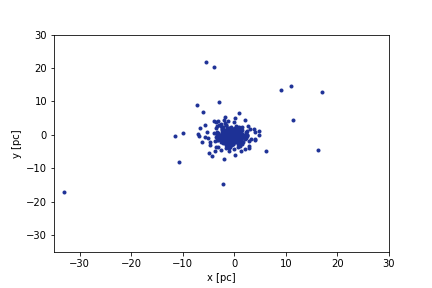
\includegraphics[width=0.5\columnwidth]{images/cluster_xy.png}
\end{center}
\caption{Proiezione di un ammasso campione sul piano del cielo.}
\label{fig:cluster}
\end{figure}
In figura \ref{fig:cluster} vi è la proiezione sul piano del cielo dell'ammasso. In figura \ref{fig:cluster1} sono riportati gli andamenti dell'accelerazione, del \textit{jerk} e dello \textit{snap} in funzione del raggio dell'ammasso. Per questi ultimi, si nota nelle regioni centrali una dispersione: probabilmente si tratta di particelle interagenti, in quanto presentano valori di accelerazione, \textit{jerk} e \textit{snap} maggiori rispetto agli andamenti generali. 
\begin{figure}[H]
\centering
\subfloat[accelerazione VS raggio]{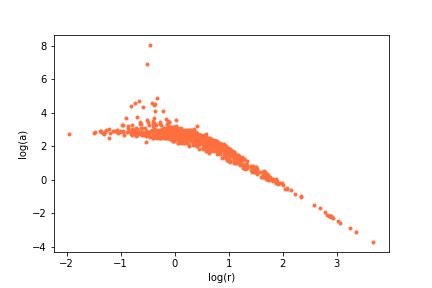
\includegraphics[width = 2.5in]{images/acc_r.png}}
\qquad
\subfloat[\textit{jerk} VS raggio]{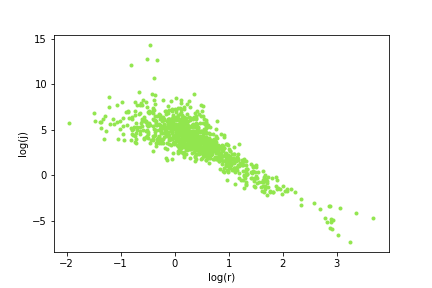
\includegraphics[width = 2.5in]{images/jerk_r.png}}
\qquad
\subfloat[\textit{snap} VS raggio]{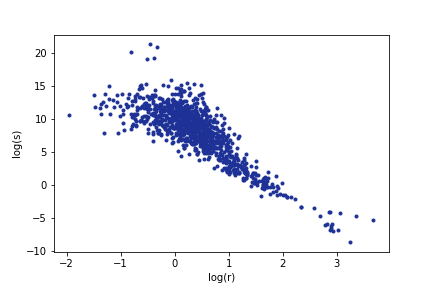
\includegraphics[width = 2.5in]{images/snap_r.png}}
\caption{Andamenti di accelerazione, \textit{jerk} e \textit{snap} in funzione del raggio delle particelle nell'ammasso campione in scala logaritmica.}
\label{fig:cluster1}
\end{figure}
In figura \ref{fig:cluster2}, invece, vi sono i \textit{jerks} e gli \textit{snaps} in funzione delle accelerazioni. Infine in figura \ref{fig:density} è riportato il profilo radiale di densità di massa dell'ammasso. Tutti i grafici sono in scala logaritmica.  
\begin{figure}[H]
\centering
\subfloat[\textit{jerk} VS accelerazione]{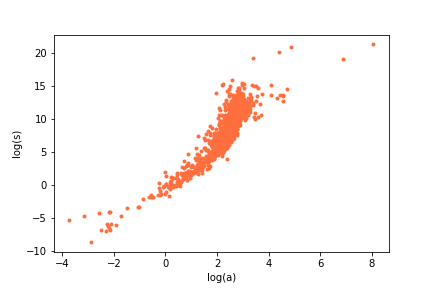
\includegraphics[width = 2.5in]{images/snap_acc.png}}
\qquad
\subfloat[\textit{snap} VS accelerazione]{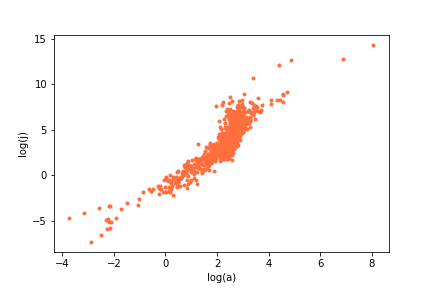
\includegraphics[width = 2.5in]{images/jerk_acc.png}}
\caption{\textit{Jerk} e \textit{snap} in funzione dell'accelerazione delle stelle dell'ammasso in scala logaritmica.}
\label{fig:cluster2}
\end{figure}
\begin{figure}[H]
\begin{center}
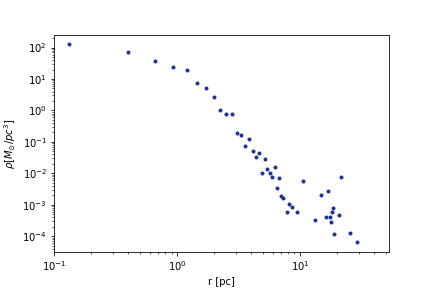
\includegraphics[width=0.5\columnwidth]{images/density.png}
\end{center}
\caption{Profilo di densità dell'ammasso in scala logaritmica.}
\label{fig:density}
\end{figure}

\section{Dataset}
Tra i risultati delle simulazioni sono stati considerati solo quelli relativi alle particelle delle zone più interne degli ammassi, in quanto, normalmente le MSPs si trovano proprio in tali regioni. 

Si è deciso di definire le zone centrali degli ammassi per mezzo del raggio che contenesse il $20\%$ delle stelle totali. Successivamente, in queste regioni, sono state eseguite 6 estrazioni casuali per ogni ammasso di un numero di MSPs variabile tra 1 e 40. Trattandosi di simulazioni che non tengono conto dell'evoluzione stellare, le particelle risultano tutte uguali, per questo motivo la scelta di estrarle casualmente è ragionevole. Tuttavia, si è scelto di selezionarle nelle regioni centrali poiché è lì che normalmente si trovano. 

I \textit{dataset} forniti all'algoritmo di ML sono in totale sei ed essi differiscono tra loro in base al diverso numero di MSPs estratte per ciascun ammasso, ovvero 1, 5, 10, 20, 30 o 40.
Pertanto, ogni \textit{record} dei diversi \textit{dataset} corrisponde ad un ammasso e, come già detto, gli ammassi simulati sono circa 200. Ciascun ammasso può contenere o meno un IMBH ed è caratterizzato da un certo numero di particelle da 1 a 40 che sono state estratte casualmente come MSPs. 

Ogni MSP è caratterizzata da posizione nell'ammasso, velocità, accelerazione, \textit{jerk} e \textit{snap}. Ma le caratteristiche delle MSPs che si è deciso di fornire come \textit{features} all'albero decisionale sono: 
\begin{itemize}
    \item il raggio proiettato sul piano del cielo, cioè la distanza di ogni particella dal centro di massa dell'ammasso: $r_{p}=\sqrt{x^{2}+y^{2}}$;
    \item la componente $z$ della velocità, $v_{z}$;
    \item la componente $z$ dell'accelerazione, $a_{z}$;
    \item la componente $z$ del \textit{jerk}, che ora indicheremo con $j_{z}$;
    \item la componente $z$ dello \textit{snap}, che indicheremo con $s_{z}$.
\end{itemize}

Sulla base di tali \textit{features} per ciascun \textit{dataset}, l'algoritmo di ML sarà in grado di predire la presenza di un IMBH negli ammassi con una certa accuratezza ed \textit{F-score}.

\section{Codice}
Il codice sviluppato per la predizione degli IMBHs al centro di GCs mediante l'utilizzo di alberi decisionali è stato scritto in Python 3.7.0 utilizzando i moduli \textbf{NumPy} \cite{numpy:online} e \textbf{scikit-learn} \cite{sklearn:online}. Esso è consultabile al seguente link di \textit{jupyter notebook}: \textbf{inserire}.

Il codice si sviluppa principalmente in quattro parti:
\begin{itemize}
    \item Fase di preparazione del \textit{dataset};
    \item Fase di addestramento sul \textit{training set};
    \item Fase di validazione;
    \item Valutazione delle prestazioni sul \textit{test set}.
\end{itemize}

Durante la prima fase, il \textit{dataset} viene diviso nei tre sottogruppi: \textit{training set}, \textit{validation set} e \textit{test set} (Sez. \ref{sec:splitdata}).
Per questo lavoro si è scelto di considerare nel \textit{test set} il $20\%$ dei dati e il restante $80\%$ viene suddiviso nel seguente modo: il $30\%$ di questi dati costituisce il \textit{validation set} ed il rimanente $70\%$ fa parte del \textit{training set}. Pertanto, il \textit{dataset} è diviso in: $56\%$ in \textit{training set}, $24\%$ in \textit{validation set} e $20\%$ in \textit{test set}. 

Nella fase successiva, l'albero decisionale di classificazione viene addestrato sul \textit{training set}. Trattandosi di un algoritmo supervisionato, quindi, gli viene fornito in input anche il vettore delle \textit{labels} in cui le due classi considerate vengono indicate con:
\begin{itemize}
    \item \textbf{classe 0 o "no"}: "non c'è un IMBH nell'ammasso";
    \item \textbf{classe 1 o "yes"}: "c'è un IMBH nell'ammasso".
\end{itemize}
Per distinguere le classi si è fissato a priori un valore di soglia per la massa. In particolare, si è decisiso di inserire nella \textbf{classe "yes"} tutti gli ammassi per cui $$\frac{M_{BH}}{M_{clus}}>0.14$$ dove con $M_{BH}$ si indica la massa del buco nero centrale e con $M_{clus}$ la massa dell'intero ammasso. Quando, invece, la massa del buco nero centrale risulta inferiore o uguale al $14\%$ della massa dell'intero ammasso, consideriamo che non ci sia un IMBH al centro dell'ammasso in questione.

Durante la fase di validazione, poi, avviene il processo di \textit{pruning} dell'albero (Sez. \ref{sec:pruning}). In questa fase si vuole scegliere il parametro di complessità $\alpha$ relativo al modello allenato per cui non si abbia \textit{overfitting}, ma che permetta di migliorare l'accuratezza delle previsioni. Come già visto in maggiore dettaglio nelle Sezioni \ref{sec:pruning} e \ref{sec:splitdata}, per ogni valore del parametro $\alpha$ che l'algoritmo fa variare in maniera crescente tra 0 e 1, esiste un'unica sottostruttura dell'albero $T$ che minimizzi la \ref{eq:costcompl}. Ad ognuno degli $\alpha$ selezionati e salvati in memoria dall'algoritmo corrisponde un modello allenato. Si vuole ora scegliere il migliore tra essi in modo da ottenere un classificatore in grado di predire in maniera accurata la presenza degli IMBHs al centro dei GCs. Per fare ciò si utilizza il \textit{validation set}. In particolare, in seguito alla fase di addestramento, il codice identifica il modello classificatore corrispondente al relativo $\alpha$ in grado di fare una predizione sul \textit{validation set} con la miglior accuratezza possibile.\\
In figura \ref{fig:acc_20part} si riporta l'andamento delle accuratezze dei modelli allenati per ciascun valore del parametro di complessità $\alpha$ in funzione del numero progressivo degli $\alpha$ stessi. Questo grafico è un esempio ottenuto a partire dal \textit{dataset} con l'estrazione di 20 MSPs per ogni ammasso, ma si è svolto lo stesso procedimento per tutti i \textit{dataset}.\\
Il modello scelto, quindi, è quello per cui si ha il massimo valore di accuratezza nelle previsioni sul \textit{validation set}.

\begin{figure}[ht]
\begin{center}
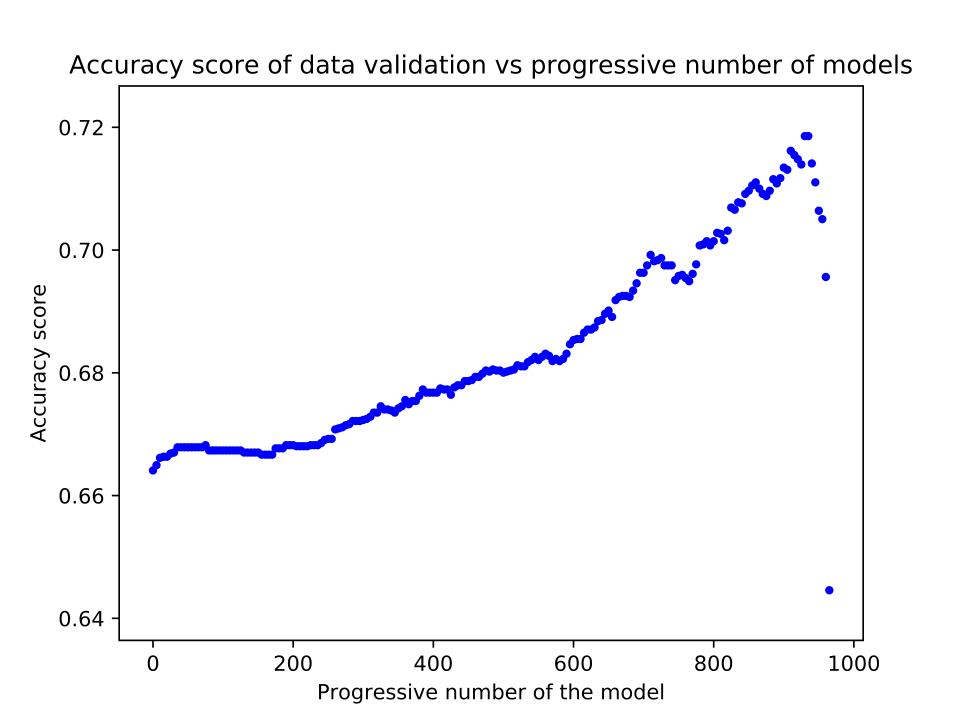
\includegraphics[width=0.7\columnwidth]{images/acc_val_20part.png}
\end{center}
\caption{Il plot è stato ottenuto a partire dal \textit{dataset} contenente 20 MSPs per ogni ammasso. Si riporta l'andamento delle accuratezze ottenute con ciascun modello allenato in funzione del numero progressivo di $\alpha$. Il modello scelto è quello che restituisce il massimo valore di accuratezza sul \textit{validation set}.}
\label{fig:acc_20part}
\end{figure}

Una volta scelto il modello, le sue prestazioni vengono valutate su un set di dati totalmente nuovi per lui: il \textit{test set}. Dopo il \textit{pruning}, infatti, il modello è in grado di classificare nuovi ammassi con una certa accuratezza senza produrre \textit{overfitting}.


\chapter{Risultati}
\label{chap:cap4}
Lo scopo principale e, se vogliamo la sfida, di ogni problema di ML consiste nell'ottenere delle buone \textit{performance} dell'algoritmo su dati nuovi e mai visti. Come descritto nel capitolo precedente, dopo aver scelto il miglior modello di albero decisionale mediante la tecnica del \textit{pruning}, bisogna valutare le sue prestazioni sul \textit{test set}. In questo Capitolo, dunque, vengono presentati i risultati ottenuti dal classificatore su ognuno dei \textit{dataset} considerati. Gli strumenti utilizzati per la valutazione sono le matrici di confusione (Sez. \ref{subsec:confmatr}) e le metriche di precisione, richiamo ed \textit{F-score}. Infine, proprio grazie alle caratteristiche degli alberi decisionali, è possibile fornire un'interpretazione dei risultati sulla base dell'\textit{importanza} delle \textit{features}.

\section{Valutazione delle performance}
Sono stati utilizzati sei \textit{dataset} diversi per la previsione della presenza di IMBHs al centro di GCs a partire dalle caratteristiche dinamiche delle MSPs che si trovano nelle regioni centrali degli ammassi. I \textit{dataset} differiscono tra loro per il numero di MSPs selezionate casualmente in queste zone per ogni ammasso: 1, 5, 10, 20, 30 o 40.

Le prestazioni degli alberi decisionali vengono valutate sui relativi \textit{test set} in base alla loro capacità nel classificare gli ammassi nella \textbf{classe 0} o nella \textbf{classe 1}.\\
In figura \ref{fig:risultati_matrici} sono riportate le matrici di confusione ottenute considerando il miglior modello classificatore per ogni \textit{dataset}. Esse sono un utile strumento per visualizzare la qualità delle classificazioni. Infatti, mettono in relazione quelli che sono i reali valori delle \textit{labels} (\textit{"True label"}) con i valori che, invece, sono stati predetti (\textit{"Predicted label"}) per ciascuna classe. Nelle celle sulle diagonali vi è il numero di risposte corrette date dal classificatore, mentre nelle altre celle vi è il numero di risposte sbagliate. Si vede che, con l'aumentare del numero di MSPs selezionate nel centro di ciascun ammasso, aumenta anche il numero di risposte corrette da parte dell'albero decisionale. In particolare, i corrispondenti valori delle metriche di precisione, richiamo ed \textit{F-score} sono riportati nelle tabelle \ref{tab:risultati_metriche}.
Per maggiore chiarezza, infine, in figura \ref{fig:f1_num}, vi è l'andamento della \textit{F-score} per ciascuna classe, in funzione del numero di MSPs considerato per ogni ammasso. Si vede che, per entrambe le classi, i valori di \textit{F-score} aumentano notevolmente (di circa il $10\%$) con l'aumentare del numero di MSPs, fino a 10 MSPs per ammasso. Da 20 MSPs in poi, le \textit{F-score} si stabilizzano al $72\%$ e $73\%$.\\
\textbf{Discussione: risultati buoni? perchè? perchè ad un certo punto la f1 si stabilizza?}

\begin{figure}[H]
\centering
\subfloat[1 MSP per ammasso.]{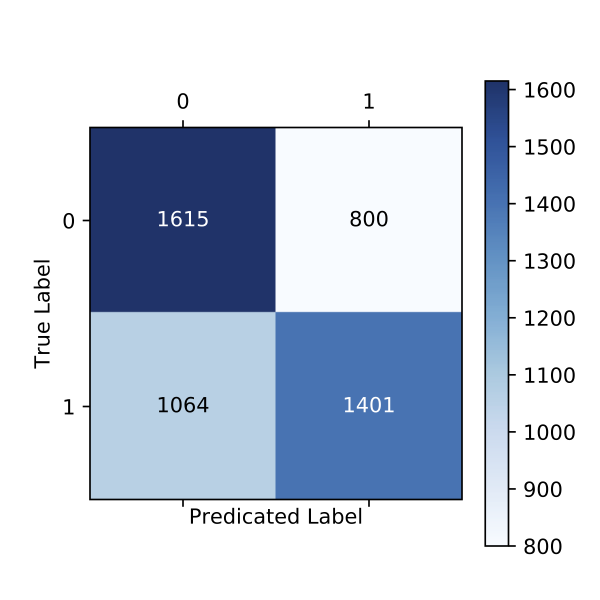
\includegraphics[width = 2in]{images/cm_1part.png}}
\qquad
\subfloat[5 MSPs per ammasso.]{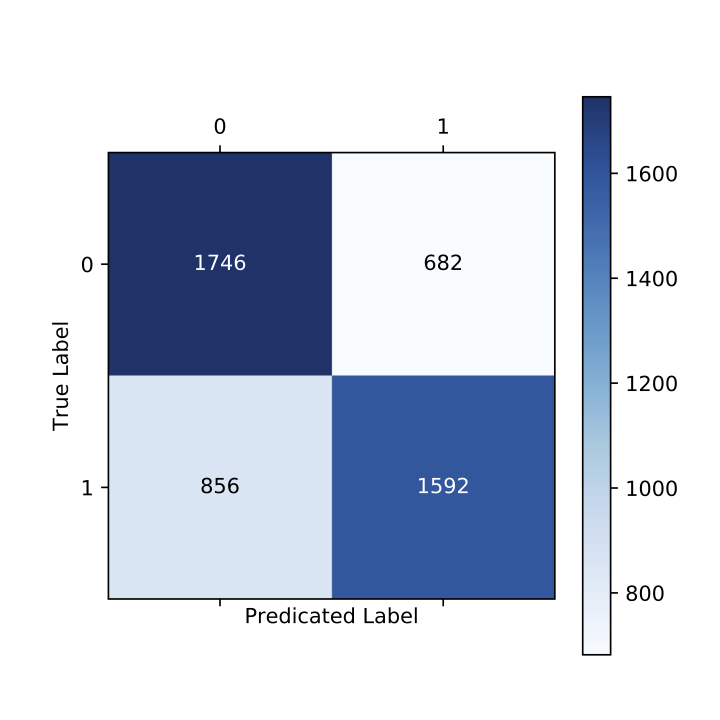
\includegraphics[width = 2in]{images/cm_5part.png}}\\
\subfloat[10 MSPs per ammasso.]{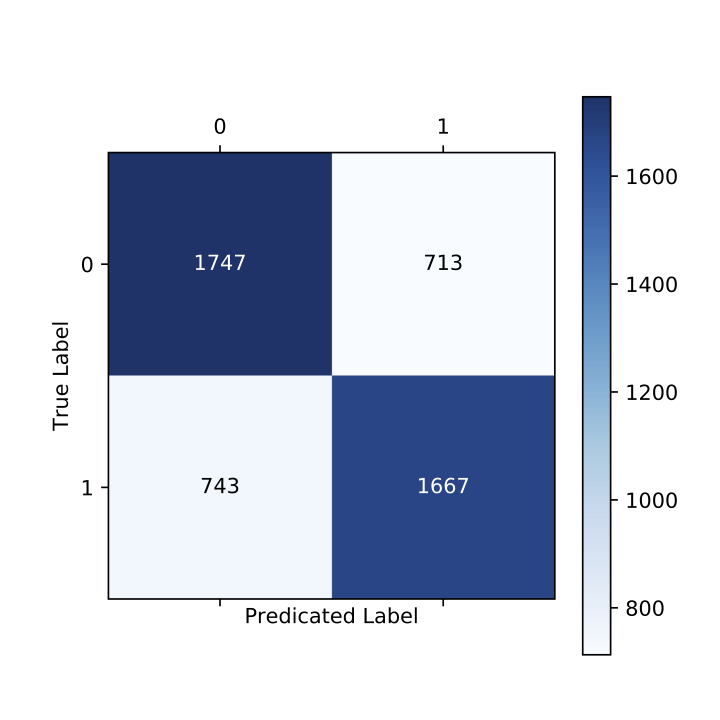
\includegraphics[width = 2in]{images/cm_10part.png}}
\qquad
\subfloat[20 MSPs per ammasso.]{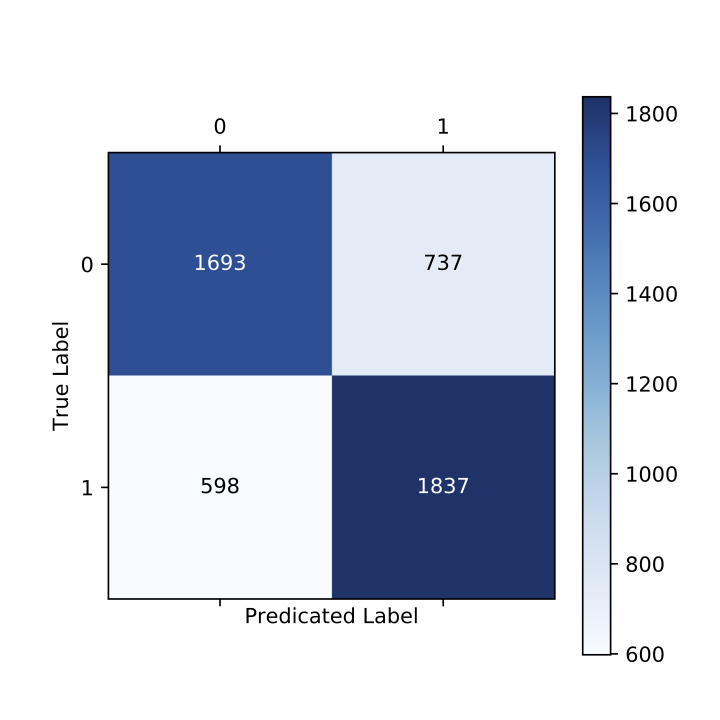
\includegraphics[width = 2in]{images/cm_20part.png}}\\
\subfloat[30 MSPs per ammasso.]{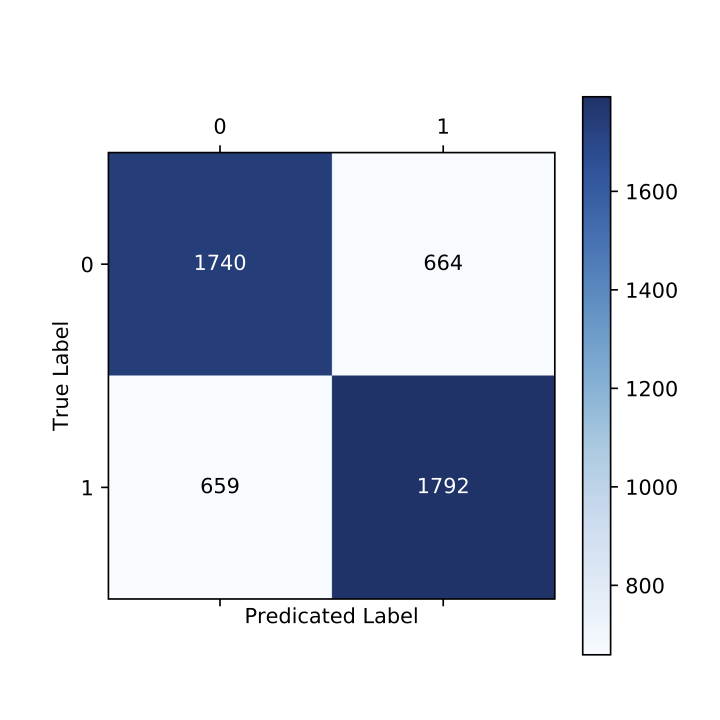
\includegraphics[width = 2in]{images/cm_30part.png}}
\qquad
\subfloat[40 MSPs per ammasso.]{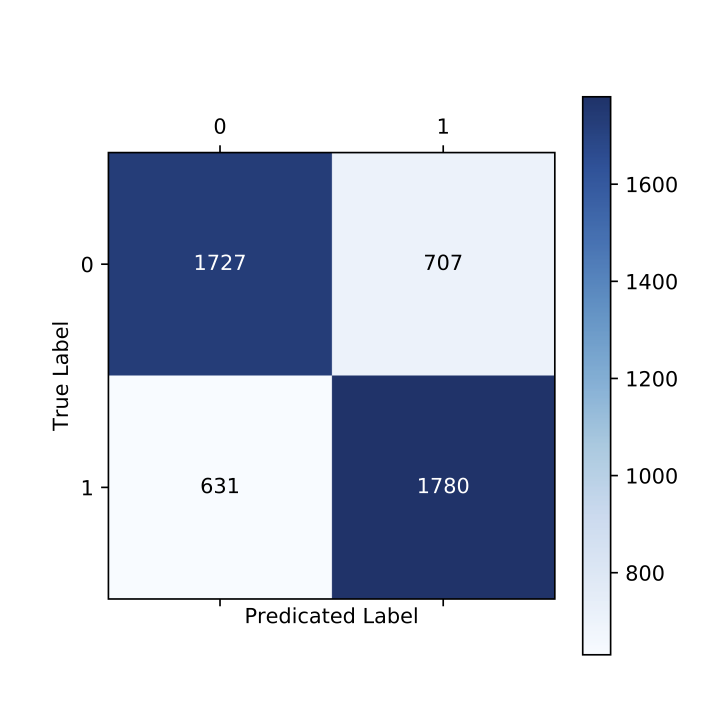
\includegraphics[width = 2in]{images/cm_40part.png}}
\caption{Matrici di confusione ottenute sui \textit{test set} per i sei diversi \textit{dataset}.}
\label{fig:risultati_matrici}
\end{figure}
\begin{table}[H]
\centering 
\subfloat[1 MSP per ammasso.]{%
	\begin{tabular}{cccc}\hline 
	classe & precisione & richiamo & F-score \\
	\hline
	0 & 0.60 & 0.67 & 0.63 \\
	\hline
	1 & 0.64 & 0.57 & 0.60\\
	\hline
	\end{tabular} 
	}
\qquad
\subfloat[5 MSPs per ammasso.]{%
	\begin{tabular}{cccc}\hline 
	classe & precisione & richiamo & F-score \\
	\hline
	0 & 0.67 & 0.72 & 0.69 \\
	\hline
	1 & 0.70 & 0.65 & 0.67\\
	\hline
	\end{tabular}} \\
\subfloat[10 MSPs per ammasso.]{%
	\begin{tabular}{cccc}\hline 
	classe & precisione & richiamo & F-score \\
	\hline
	0 & 0.70 & 0.71 & 0.71 \\
	\hline
	1 & 0.70 & 0.69 & 0.70\\
	\hline
	\end{tabular} 
		} 
\qquad
\subfloat[20 MSPs per ammasso.]{%
	\begin{tabular}{cccc}\hline 
	classe & precisione & richiamo & F-score \\
	\hline
	0 & 0.74 & 0.70 & 0.72  \\
	\hline
	1 & 0.71 & 0.75 & 0.73\\
	\hline
	\end{tabular}} \\
\subfloat[30 MSPs per ammasso.]{%
	\begin{tabular}{cccc}\hline 
	classe & precisione & richiamo & F-score \\
	\hline
	0 & 0.73 & 0.72 & 0.72 \\
	\hline
	1 & 0.73 & 0.73 & 0.73\\
	\hline
	\end{tabular} 
		}
\qquad
\subfloat[40 MSPs per ammasso.]{%
	\begin{tabular}{cccc}\hline 
	classe & precisione & richiamo & F-score \\
	\hline
	0 & 0.73 & 0.71 & 0.72 \\
	\hline
	1 & 0.72 & 0.74 & 0.73\\
	\hline
	\end{tabular}} \\
\caption{Risultati di precisione, richiamo ed F-score per ciascuna classe, ottenuti sui \textit{test set} per i sei diversi \textit{dataset}.} 
\label{tab:risultati_metriche}
\end{table}

\begin{figure}[H]
\begin{center}
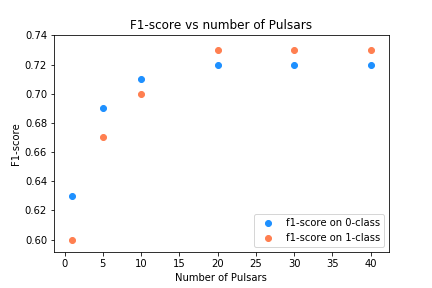
\includegraphics[width=1\columnwidth]{images/f1_num.png}
\end{center}
\caption{Andamento della \textit{F-score} per le due distinte classi in funzione del numero di MSPs considerate per ogni ammasso.}
\label{fig:f1_num}
\end{figure}

\section{Interprtazione dei risultati}
Gli alberi decisionali, soprattutto se non sono molto profondi, sono semplici da interpretare, in quanto essi possono essere visualizzati.\\
In figura \ref{fig:tree_1part} è riportato un esempio di albero decisionale ottenuto con il \textit{dataset} relativo ad una MSP estratta per ogni ammasso.

L'interpretazione è semplice: partendo dal nodo radice si percorre l'albero passando per i nodi successivi per mezzo dei rami. Questi ultimi suggeriscono quale sottoinsime andremo a guardare. Abbiamo già visto che gli \textit{split}, per ogni sottoinsieme, vengono decisi in base ad una misura di impurità fatta sulla valutazione dell'indice di Gini.\\ L'algoritmo sceglie come nodo radice quello con impurità più bassa, ossia quello con il valore di indice di Gini minore.\\ Una volta deciso il nodo radice, l’albero viene ingrandito ad una profondità pari ad uno. Lo stesso processo viene ripetuto per gli altri nodi nell’albero fino a raggiungere la massima profondità. In questo caso, stiamo interpretando un albero con profondità pari a 7, ottenuta in seguito alla fase di potatura.
\begin{figure}[H]
\begin{center}
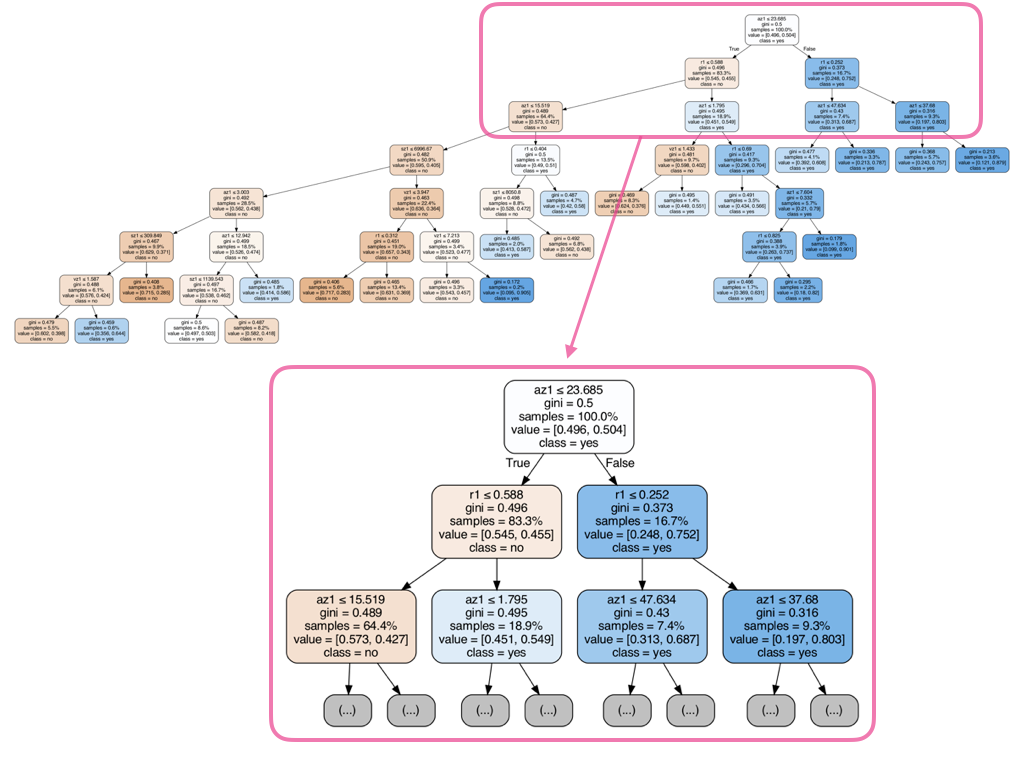
\includegraphics[width=1.1\columnwidth]{images/tree_1part_ok.png}
\end{center}
\caption{Un esempio di albero decisionale ottenuto a partire dal \textit{dataset} di 1 MSP selezionata nella regione centrale di ogni ammasso considerato. Per chiarezza è stato eseguito uno zoom nei primi \textit{split} dell'albero.}
\label{fig:tree_1part}
\end{figure}
Per maggior chiarezza, in figura \ref{fig:tree_1part} è stato fatto uno zoom sui primi \textit{split}, in particolare per il primo nodo abbiamo che:
\begin{itemize}
    \item $\mathbf{a_{z1} \le 23.685}$: il primo \textit{split} viene fatto sulla \textit{feature} $a_{z1}$, ovvero ci si chiede se essa è minore o uguale di 23.685 e, in base al risultato, si segue il percorso \textit{True} (freccia di sinistra) o \textit{False} (freccia di destra);
    \item $\mathbf{gini = 0.5}$: è l'indice di Gini per la \textit{feature} $a_{z1}$. Un valore dell'indice di Gini pari a 0 significa che il nodo è puro, ossia che esiste solo una classe (quindi che gli ammassi appartengono tutti alla \textbf{classe “yes”} o alla \textbf{classe “no”}). Al contrario, un valore maggiore di 0, come nel nodo radice, ci indica che i campioni all’interno del nodo appartengono ad entrambe le classi; 
    \item $\mathbf{samples = 100\%}$: indica la percentuale di ammassi da classificare appartenenti al \textit{training set}. Nel nodo radice è corretto aspettarsi che ancora tutti gli ammassi devono essere classificati;
    \item $\mathbf{value = [0.496, 0.504]}$: indica la frazione di ammassi di quel nodo che ricadono in ciascuna classe. Ciò significa che nel nodo radice il $49.6\%$ degli ammassi appartiene alla \textbf{classe "no"} (che abbiamo anche chiamato \textbf{classe 0}) ed il restante $50.4\%$ fa parte della \textbf{classe "yes"} (chiamata anche \textbf{classe 1});
    \item $\mathbf{class = yes}$: rappresenta la previsione su quel determinato nodo e si ricava da \textbf{value}. Infatti, dal punto sopra, capiamo che nel nodo c'è una percentuale maggiore di campioni appartenenti alla \textbf{classe “yes”}.
\end{itemize}
Queste denominazioni vengono ripetute per i vari nodi successivi dell’albero. Nello specifico, si può notare che la somma delle \textit{samples} dei nodi figli restituisce il valore \textit{samples} dei nodi padri.\\
Inoltre, la \textbf{classe "yes"} è identificata con l'azzurro, mentre la \textbf{classe "no"} con l'arancione. L'intensità della colorazione di ogni nodo varia in base all'accuratezza della previsione: vediamo che nei nodi di azzurro più intenso una percentuale maggiore di ammassi viene classificata in \textbf{"yes"} e in quelli di arancione più intenso, invece, una percentuale maggiore di ammassi viene classificata in \textbf{"no"}.\\
Infine, nei nodi foglia non appaiono più le \textit{features}, in quanto si è raggiunta la massima profondità e tutti gli ammassi in quel nodo, sono stati classificati.

In ultimo, è possibile valutare l'importanza delle diverse \textit{features} per un albero decisionale. L'importanza complessiva di una singola \textit{feature} può essere calcolata nel modo seguente: bisogna esaminare tutti gli \textit{split} per i quali la \textit{feature} è stata utilizzata e misurare quanto essa ha ridotto l'indice di Gini rispetto al nodo padre. La somma di tutte le importanza viene scalata a 100, pertanto, ogni importanza può essere interpretata come una quota dell'importanza complessiva per il modello \cite{molnar2019:book}. Nelle figure \ref{fig:importanze} e \ref{fig:importanze1} vengono riportati gli istogrammi relativi alle importanze delle diverse \textit{features} per ciascuno dei \textit{dataset} utilizzati. Le MSPs sono ordinate per raggi $r_{p}$ proiettati sul piano del cielo crescenti. E, le altre \textit{features} sono i rispettivi valori di velocità $v_z$, accelerazione $a_z$, \textit{jerk} $j_z$ e \textit{snap} $s_z$ delle MSPs lungo la linea di vista. Si può notare che, in tutti i casi, le \textit{features} con importanza maggiore sono: i raggi, in particolare quello dell'ultima MSP, le accelerazioni e gli \textit{snap}.\\
Che le accelerazioni fossero caratterizzate da un'alta importanza era un risultato atteso. Una possibile spiegazione, invece, per l'importanza del raggio dell'ultima MSP potrebbe essere che il modello lo interpreti come una misura della dimensione dell'ammasso, o meglio, come la distanza che delimita lo spazio in cui si trovano le MSPs considerate.\\
Per quanto riguarda, infine, velocità e \textit{jerks}, ossia le derivate dispari delle posizioni, essi sembra che non abbiano importanza per il modello \textbf{perchè?}

\begin{figure}[H]
\centering
\subfloat[1 MSP per ammasso.]{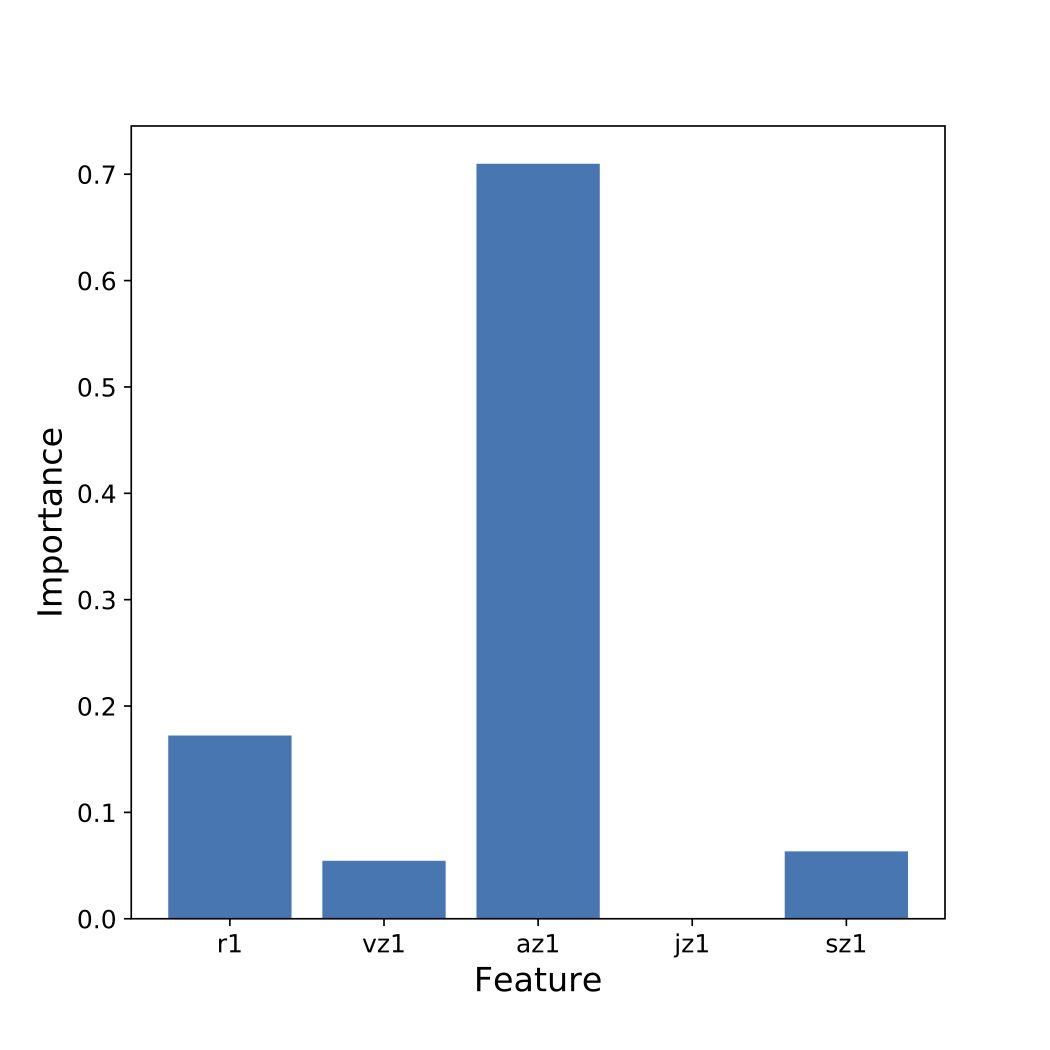
\includegraphics[width = 3in]{images/bar_imp_1part.png}}\\

\subfloat[5 MSPs per ammasso.]{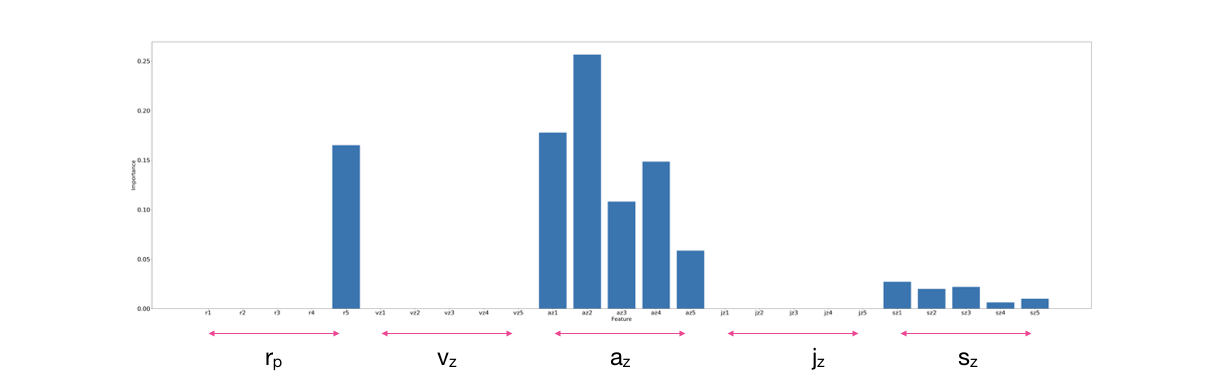
\includegraphics[width = 6in]{images/bar_imp_5part.png}}\\

\subfloat[10 MSPs per ammasso.]{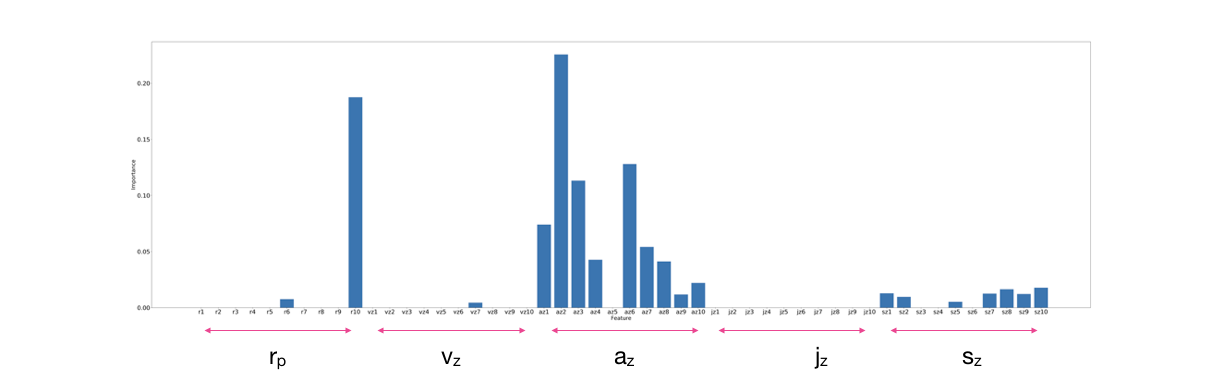
\includegraphics[width = 6in]{images/bar_imp_10part.png}}
\caption{Grafici delle importanze delle \textit{features} per il modello calcolate per i \textit{dataset} relativi a 1, 5 e 10 MSPs per ammasso (dall'alto verso il basso).}
\label{fig:importanze}
\end{figure}

\begin{figure}[H]
\centering
\subfloat[20 MSPs per ammasso.]{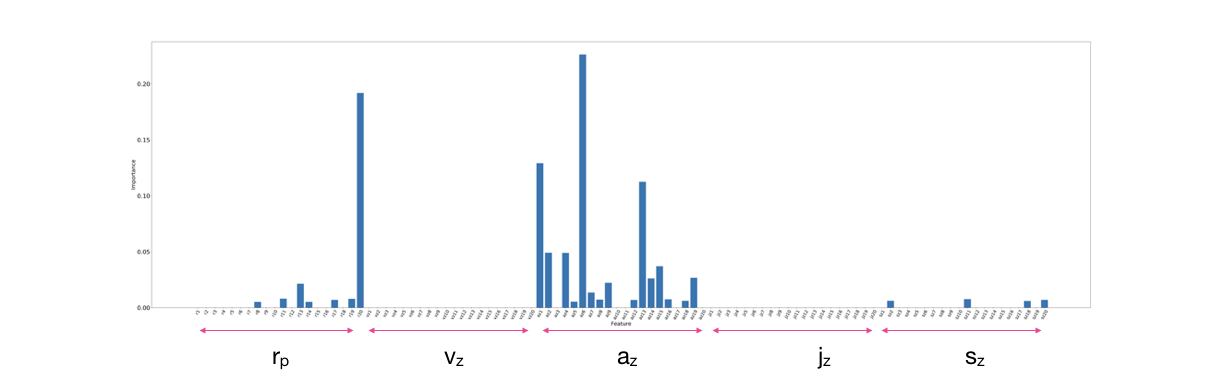
\includegraphics[width = 6in]{images/bar_imp_20part.png}}\\

\subfloat[30 MSPs per ammasso.]{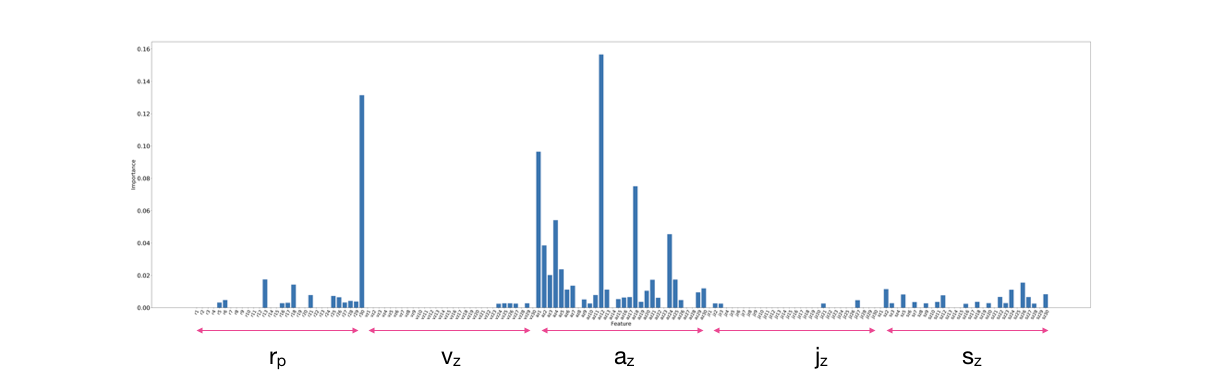
\includegraphics[width = 6in]{images/bar_imp_30part.png}}\\

\subfloat[40 MSPs per ammasso.]{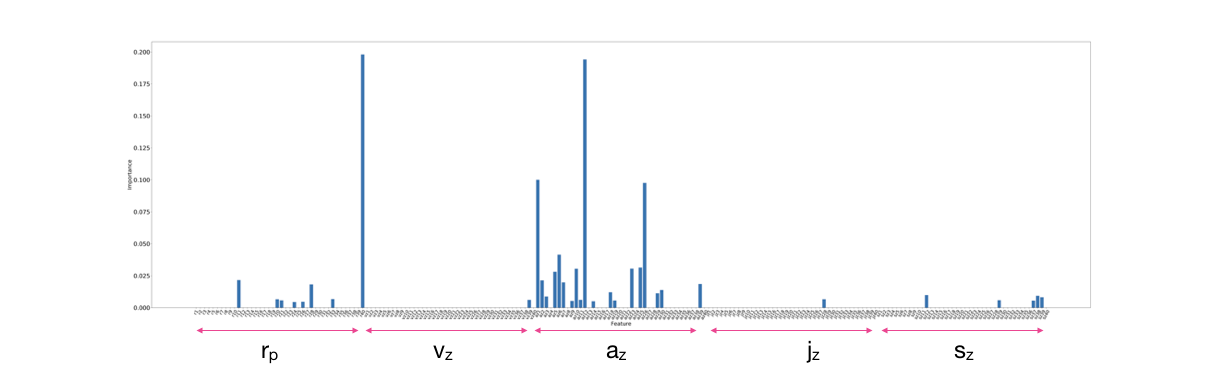
\includegraphics[width = 6in]{images/bar_imp_40part.png}}
\caption{Grafici delle importanze delle \textit{features} per il modello calcolate per i \textit{dataset} relativi a 20, 30 e 40 MSPs per ammasso (dall'alto verso il basso).}
\label{fig:importanze1}
\end{figure}



\chapter{Conclusioni e sviluppi futuri}
\label{chap:cap5}
Gli IMBHs, la loro esistenza ed il fatto di poterli trovare al centro dei GCs sono stati per lungo tempo oggetto di dibattito nel mondo scientifico.
I modelli teorici attuali indicano che è possibile identificarli negli ammassi globulari, mentre i metodi osservativi usati finora non ne hanno ancora verificato la presenza. Un interessante metodo proposto per identificarli è quello che si basa sullo studio dinamico delle MSPs in ammasso. Da qui nasce l'idea di questo lavoro di tesi: voler identificare gli IMBHs in ammassi globulari attraverso una tecnica di ML interpretabile utilizzando le caratteristiche dinamiche delle MSPs. Si tratta, infatti, di voler applicare un metodo nuovo ad un problema ben noto.

A partire dai risultati di un set di simulazioni a N-corpi di ammassi globulari sono stati creati i \textit{dataset} forniti all'algoritmo di ML. Lo scopo è stato quello di voler prevedere la presenza di IMBHs in questi ammassi sulla base della posizione nel piano del cielo delle MSPs e delle loro componenti lungo la linea di vista di velocità, accelerazione, \textit{jerk} e \textit{snap}. Per farlo ci si è serviti degli alberi decisionali.\\
Sono stati considerati circa 200 ammassi, per ognuno dei quali sono state effettuate 6 estrazioni casuali di un numero variabile tra 1 e 40 di MSPs selezionate casualmente dalle regioni centrali degli ammassi stessi. 

Nonostante gli alberi decisionali non siano tra i modelli di ML più sofisticati, si ottengono dei buoni risultati. In particolare, si riescono a classificare gli ammassi in base alla presenza di un IMBH con valori di accuratezza pari a circa il $70\%$.\\ 
Inoltre, la caratteristica fondamentale degli alberi decisionali è che essi possono essere facilmente interpretati, specie quando si tratta di alberi non molto profondi. Per questo motivo, questi modelli vengono spesso preferiti rispetto ad altri.\\
Dall'interpretazione delle scelte che il modello compie in ogni nodo dell'albero è possibile capire quali sono state le caratteristiche dinamiche delle MSPs che hanno avuto più importanza nella fase di allenamento del modello. Per tutti i casi analizzati risulta che, come atteso, l'importanza maggiore viene attribuita alle accelerazioni delle MSPs negli ammassi. Molto importante risulta anche il raggio proietatto sul piano del cielo della MSP più distante. Il resto delle importanze è distribuito tra gli \textit{snaps} ed i raggi proiettati delle altre MSPs.

Nella pratica, dopo aver monitorato un certo numero di MSPs in un ammasso misurandone le caratteristiche dinamiche, quello che si vuole capire è se, in base ai loro valori, l'ammasso possa ospitare un IMBH o meno. Se in questa fase avessimo già allenato un modello di ML a partire da dati di sumilazioni, allora si potrebbe prevedere nella realtà la presenza di tali oggetti tanto ricercati.\\ L'importanza di questo lavoro sta proprio nel fatto che sarebbe possibile ottenere un riscontro futuro su dati veri. Per tale ragione, sarebbe fondamentale affinare questo modello e svilupparne altri a partire da questo, per ottenere previsioni più accurate.\\
Un primo passo verso il miglioramento delle \textit{performance} dell'algoritmo è quello di rendere le simulazioni da cui provengono i \textit{dataset} il più verosimili possibile, ad esempio considerando anche l'evoluzione stellare. In secondo luogo, invece, si potrebbero migliorare alcuni punti importanti del codice di previsione. Infatti, il criterio considerato per determinare la presenza di un IMBH in un ammasso si basa su un valore di soglia di massa relativa scelto a priori. Questo passaggio è cruciale per la classificazione degli ammassi nelle due distinte classi, per questo sarebbe importante svolgere, in futuro, uno studio più approfondito sulla scelta di tale criterio (\textbf{suggerimenti su un possibile metodo?}).

Infine, è lecito sostenere che l'originalità di questo studio stia proprio nei metodi applicati ad una questione astrofisica ormai nota. Per questo sarebbe importante concentrarsi sui suoi possibili sviluppi e miglioramenti, con la prospettiva che possa essere utile per ricerche future.


\appendix
% INCLUSIONE APPENDICI - - PERSONALIZZARE - TENERE COERENTE CON LISTA IN ALTO
%\chapter{An appendix}
\label{app:a}


%%%%%%%%%%%%%%%%%%%%%%%%%%%%%%%%%%%%%%%%%%%%%%%%%%%%%%%%%%%%%%%

% BIBLIOGRAFIA
\phantomsection
\addcontentsline{toc}{chapter}{\refname}
\nocite{*}
\printbibliography

\end{document}
